\documentclass[]{article}
% bib use
\usepackage{cite}
% tabular eqn
\usepackage{amsmath, array}
% code listing
\usepackage{listings}
% images
\usepackage{graphicx} 
% lock images
\usepackage{float}
% colored syntax highlighting
\usepackage{xcolor}  
%captions in listings
\usepackage{caption}
% multirows in tables
\usepackage{multirow}
%longtable
\usepackage{array}
\usepackage{longtable}
%mathbb
\usepackage{amsfonts}


%opening
\title{Principles of statistical inference project - Part 2}
\author{Carmel Gafa}

\begin{document}

\maketitle

% style for all code snippets
\lstset{
	basicstyle=\ttfamily\footnotesize,  % Use Courier (monospace)
	numbers=left, numberstyle=\tiny, stepnumber=1, numbersep=5pt,
	breaklines=true, breakatwhitespace=true,
	frame=single, rulecolor=\color{gray}  % Single-line frame
}


\section{Question 1}

\textbf{Find and download a dataset from the internet that includes at least three quantitative
variables (more is better). Once you have selected a dataset, send the link via email to Dr.
Monique Borg Inguanez (monique.inguanez@um.edu.mt) for approval, ensuring that each
student works with a unique dataset.
Using the approved dataset, fit a Bayesian multiple linear regression model ($p < 2$) using
JAGS.
Your submission should clearly include the following:}

\bigskip

The selected dataset is the Concrete Compressive Strength dataset, which was downloaded from the University of California, Irvine. The response variable of the dataset is the Concrete compressive strength as a function of eight predictors, including ingredients and ageing time.

The following table outlines the variables of the dataset, which had no missing values:

\begin{table}[H]
	\centering
	\begin{tabular}{|l|l|l|l|}
		\hline
		\textbf{Variable Name} & \textbf{Role} & \textbf{Type} & \textbf{Units} \\ \hline
		Cement                 & Feature       & Continuous     & kg/m\textsuperscript{3} \\ \hline
		Blast Furnace Slag     & Feature       & Integer        & kg/m\textsuperscript{3} \\ \hline
		Fly \texttt{ash}                & Feature       & Continuous     & kg/m\textsuperscript{3} \\ \hline
		Water                  & Feature       & Continuous     & kg/m\textsuperscript{3} \\ \hline
		Superplasticizer       & Feature       & Continuous     & kg/m\textsuperscript{3} \\ \hline
		Coarse Aggregate       & Feature       & Continuous     & kg/m\textsuperscript{3} \\ \hline
		Fine Aggregate         & Feature       & Continuous     & kg/m\textsuperscript{3} \\ \hline
		Age                    & Feature       & Integer        & day \\ \hline
		Concrete Compressive Strength & Target & Continuous     & MPa \\ \hline
	\end{tabular}
	\caption{Variables in the Concrete Compressive Strength dataset}
	\label{tab:concrete_variables}
\end{table}

A first test on the dataset involved a pairwise and visual inspection of the relationships to determine the correlation of the predictors with the response and to start forming some ideas about multicollinearity. These results are shown below in Figure \ref{fig:img-pairwise-numeric} and Figure \ref{fig:img-pairwise-plot}.



\begin{figure}[H]
	\centering
	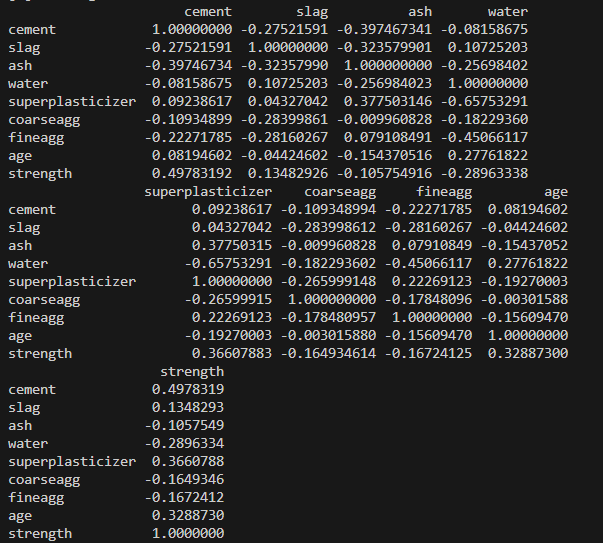
\includegraphics[width=0.5\linewidth]{img/img-pairwise-numeric}
	\caption{ Correlation matrix of all variables in the Concrete Compressive Strength dataset. }
	\label{fig:img-pairwise-numeric}
\end{figure}


\begin{figure}[H]
	\centering
	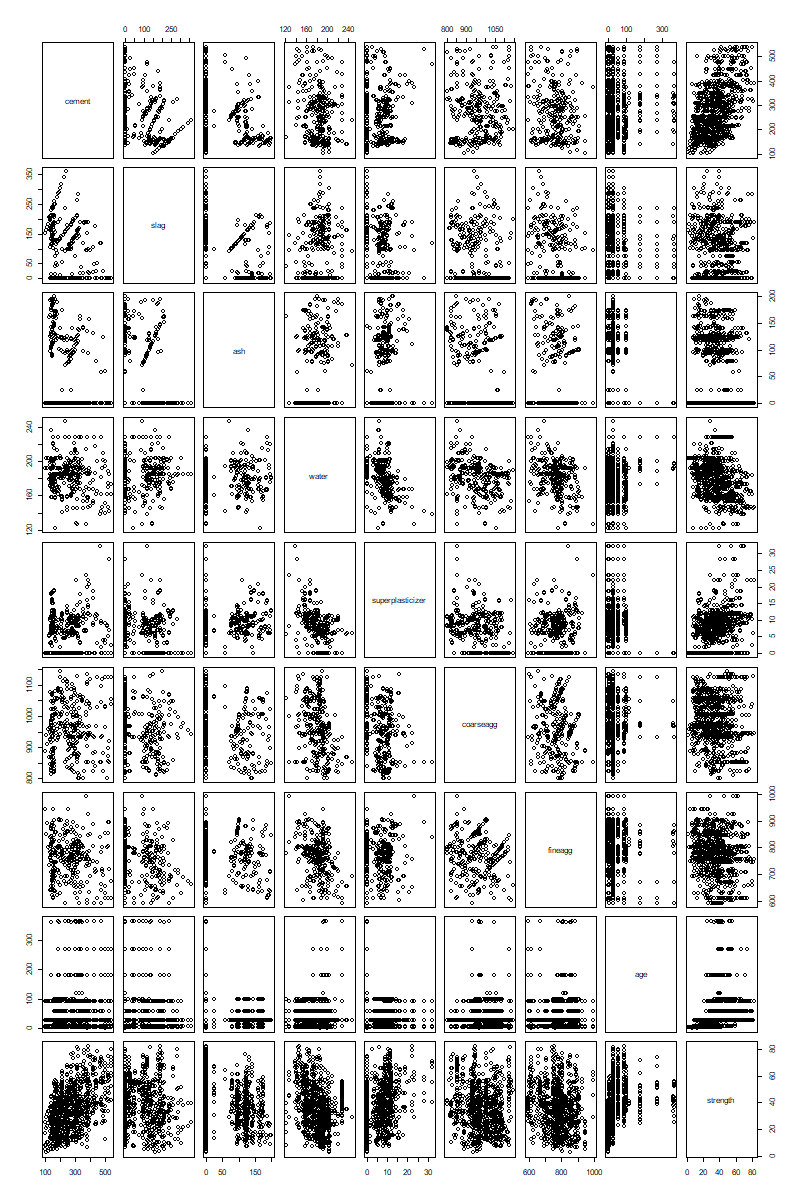
\includegraphics[width=0.5\linewidth]{img/img-pairwise-plot}
	\caption{Pairwise scatterplot matrix of all variables in the Concrete Compressive Strength dataset.}
	\label{fig:img-pairwise-plot}
\end{figure}


From this result, the best correlation with strength is achieved with \texttt{cement}, followed by a moderate correlation with \texttt{superplasticiser} (+0.37) and \texttt{age} (+0.33).
Water has a moderate negative correlation (-0.29). \texttt{Slag} and \texttt{ash} have a weak correlation. We can also see a strong negative correlation between \texttt{superplasticiser} and \texttt{water} (-0.66) and \texttt{water} and \texttt{fine aggregate} (-0.45).


Variance inflation factor analysis was then conducted to investigate multicollinearity, with the results of the analysis presented in Figure \ref{fig:img-vif}.

\begin{figure}
	\centering
	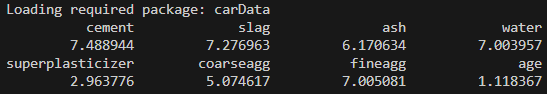
\includegraphics[width=0.7\linewidth]{img/img-vif}
	\caption{Variance Inflation Factor values for all predictors in the Concrete Compressive Strength dataset.}
	\label{fig:img-vif}
\end{figure}



The analysis shows that cement,  \texttt{Slag}, \texttt{ash}, and \texttt{water} exhibit high collinearity (in the region of 7), while \texttt{superplasticiser} (2.96) and  \texttt{age} (1.12) have moderate values.

Following this investigation, cement, \texttt{superplasticiser}, and \texttt{age} were selected as predictors.


The following code snippet illustrates the data preparation. Prior to this step, the datasets's column names were shortened so they could be manipulated easily.

\begin{lstlisting}
script_dir <- getwd()
concrete_cleansed_path <- file.path(
script_dir, "project_2_code/concrete_cleansed.csv")

concrete_cleansed <- read.csv(concrete_cleansed_path)

jags_data <- list(
x_cement = concrete_cleansed$cement,
x_superplasticizer = concrete_cleansed$superplasticizer,
x_age = concrete_cleansed$age,
y_strength = concrete_cleansed$strength,
n = nrow(concrete_cleansed)
)
\end{lstlisting}




\subsection{A full specification of the Bayesian model:}
\textbf{\begin{itemize}
	\item The likelihood function
	\item The prior distributions selected for the parameters
\end{itemize}}



The response variable in this excercise is \texttt{strength}, representing the concrete compressive strength in MPa. As we have seen in the previous section, the predictors included in the model are \texttt{cement}, \texttt{superplasticizer}, and \texttt{age}, all selected based on correlation and multicollinearity analysis.

The model assumes the following structure:

\begin{flalign*}
	y_i &\sim \mathcal{N}(\mu_i, \tau^{-1}) \quad \text{for } i = 1, \dots, n \\
	\mu_i &= \beta_0 + \beta_1 \cdot x_{\text{cement}, i} + \beta_2 \cdot x_{\text{superplasticizer}, i} + \beta_3 \cdot x_{\text{age}, i}
\end{flalign*}

The prior distributions for the parameters are defined as follows:

\begin{align*}
	\beta_0 &\sim \mathcal{N}(0, 100) \\
	\beta_1 &\sim \mathcal{N}(0, 100) \\
	\beta_2 &\sim \mathcal{N}(0, 100) \\
	\beta_3 &\sim \mathcal{N}(0, 100) \\
	\tau &\sim \text{Gamma}(0.01, 0.01)
\end{align*}

The variance of the likelihood is modeled via the precision parameter $\tau$, where;
$$
\tau = \frac{1}{\sigma^2}
$$

The model was defined using the following statement:

\begin{lstlisting}
model_description <- "
model {
	for (i in 1:n) {
		y_strength[i] ~ dnorm(mu[i], tau)
		mu[i] <- beta0 + (beta1 * x_cement[i]) + (beta2 * x_superplasticizer[i]) + (beta3 * x_age[i])
	}
	beta0 ~ dnorm(0, 0.01)
	beta1 ~ dnorm(0, 0.01)
	beta2 ~ dnorm(0, 0.01)
	beta3 ~ dnorm(0, 0.01)
	tau ~ dgamma(0.01, 0.01)
} "
		
\end{lstlisting}



\subsection{A justification for the chosen priors, including any assumptions or reasoning behind
them.}


The priors in this model are weakly informative; that is, they do not strongly influence the results, but they give only a little information about what values we expect for the parameters. The coefficients for $\beta$, for example, were given normal priors centred at 0 with a standard deviation of 10, which allows for a large range of possible values. These priors are wide enough to let the data have the biggest impact on the results, but they also help the model stay stable and avoid extreme or unrealistic values during sampling.

\begin{itemize}
	\item \textbf{Regression Coefficients ($\beta_0$, $\beta_1$, $\beta_2$, $\beta_3$):} Each coefficient was assigned a normal prior $\mathcal{N}(0, 100)$, corresponding to a mean of 0 and a large variance of 100, reflecting a belief that the effect of each predictor is centred around zero but allows for a wide range of plausible values. As discussed, these priors are considered weakly informative because they do not strongly constrain the parameter estimates but prevent extreme values that could destabilize the sampling process.
	
	\item \textbf{Precision Parameter ($\tau$):} A Gamma$(0.01, 0.01)$ prior was used for the precision of the normal likelihood, which is a standard weak prior for precision in Bayesian models. It gives a very wide range of possible values for the standard deviation, which means we do not assume much about how spread out the data is, reflecting that we have little prior knowledge about the variation in the response.
\end{itemize}

The priors were selected to reflect minimal assumptions about the parameter values in the absence of strong domain knowledge, which is appropriate given the exploratory nature of this analysis.

\subsection{The selected burn-in period for your MCMC chains, including a detailed explanation
of how this was chosen.}

%In Bayesian analysis using Markov Chain Monte Carlo, the initial samples of each chain will, in most cases, not reflect the target posterior distribution, and the chain will settle into the posterior distribution after a number of samples. This early phase is known as the burn-in period. These initial samples are discarded before subsequent analysis, as they would bias the results.

Trace plots are the first tool that is used to determine a suitable burn-in period. In this analysis, we examine chain mixing, which the overlap of the chain samples can visually assess, and compactness within the chain samples. Additionally, chain variations should be consistent around a central value. Trace plots, however, are subjective in interpretation and can indicate early convergence. Another tool that is then used is the Gelman-Rubin convergence diagnostic, which utilises both between-chain and within-chain variance to assess convergence.

Figure~\ref{fig:img-trace-beta0} shows the trace plot for the parameter $\beta_0$, that is, the intercept after a burn-in of just 200 samples. The trance can visually satisfy the criteria for convergence.

\begin{figure}[H]
	\centering
	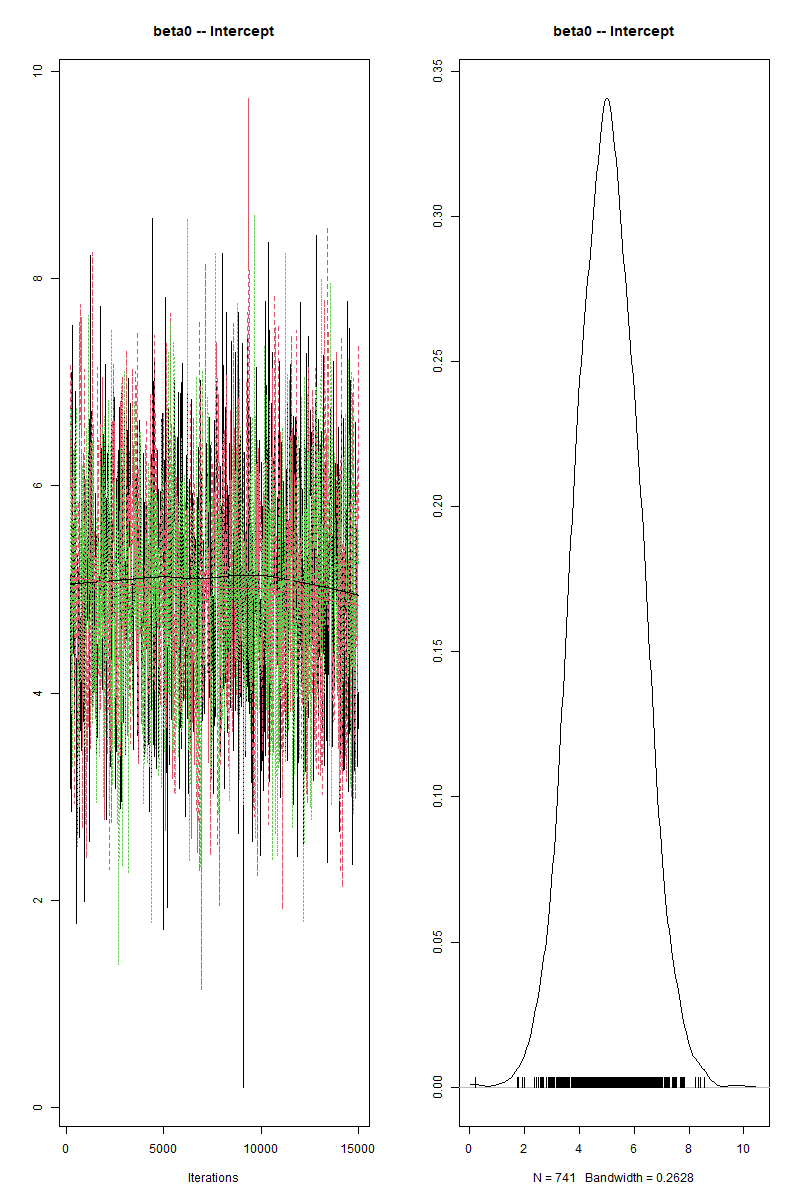
\includegraphics[width=0.7\linewidth]{img/img-trace-beta0}
	\caption{Trace and density plot for $\beta_0$ (Intercept) across 3 chains after iteration 200.}
	\label{fig:img-trace-beta0}
\end{figure}


The Gelman-Rubin diagnostic was also examined. Figure~\ref{fig:img-gelman-plot-beta0} shows that the values for all parameters converge to 1.00 after iteration 6000, confirming chain convergence and the initial iterations were likely influenced by starting values.

\begin{figure}[H]
	\centering
	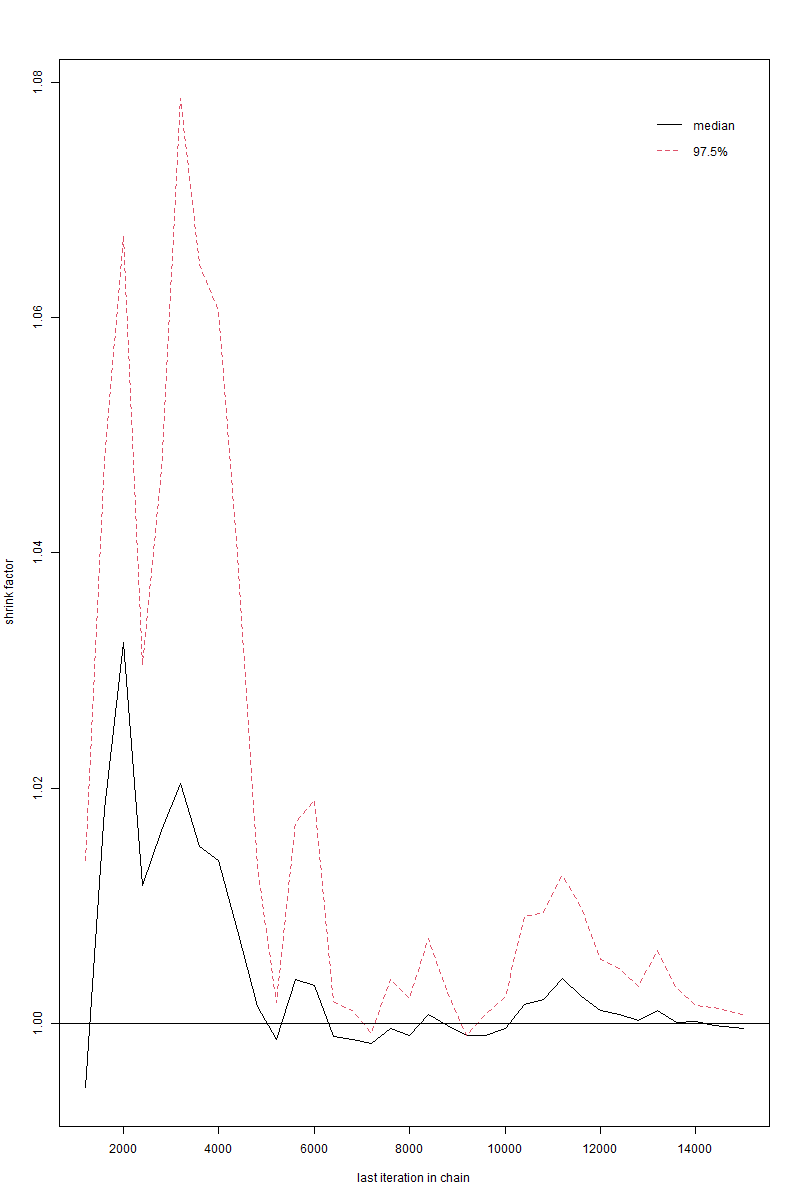
\includegraphics[width=0.7\linewidth]{img/img-gelman-plot-beta0}
	\caption{Gelman--Rubin diagnostic for $\beta_0$. Convergence is reached after approximately 6000 iterations}
	\label{fig:img-gelman-plot-beta0}
\end{figure}


Based on these observations, a burn-in of 6000 iterations was selected to ensure that only samples drawn from the stationary portion of the chains were retained for posterior inference.


The following snippet shows the execution of the model and creation of the plot used in this analysis

\begin{lstlisting}
n_chains <- 3
n_burnin <- 200
n_samples <- 15000
parameters_to_monitor <- c("beta0", "beta1", "beta2", "beta3", "tau")

initial_values <- list(
list(beta0 = -10, beta1 = 0.5, beta2 = 0.1, beta3 = 0.05, tau = 0.5),
list(beta0 = 0,   beta1 = 1,   beta2 = 0.3, beta3 = 0.1,  tau = 1),
list(beta0 = 10,  beta1 = 2,   beta2 = 0.5, beta3 = 0.2,  tau = 2)
)

model <- jags.model(textConnection(model_description),
data = jags_data,
inits = initial_values,
n.chains = n_chains)

post <- coda.samples(model = model,
variable.names = parameters_to_monitor,
n.iter = n_samples,
thin = 20)

post_burned <- window(post, start = n_burnin)
print(summary(post_burned))
plot(post_burned[, "beta0"], main="beta0 -- Intercept")
\end{lstlisting}



\subsection{A presentation and interpretation of:}
\textbf{\begin{itemize}
	\item Convergence diagnostics (e.g., trace plots, Gelman-Rubin statistics)
	\item Accuracy diagnostics (e.g., effective sample size, autocorrelation)
\end{itemize}}


The Figures below illustrate convergence diagnostics for all monitored parameters in the model. Trace plots are shown after discarding an initial burn-in of 200 samples, highlighting chain behaviour and visual mixing. Additionally, Gelman-Rubin diagnostic plots are presented both after a burn-in of 200 samples and after a more conservative burn-in of 6000 samples. These plots allow for a comparative evaluation of convergence, confirming that the longer burn-in more effectively removed transient behaviour and yielded PSRF values stabilising around 1.00 across all parameters.


\begin{figure}[H]
	\centering
	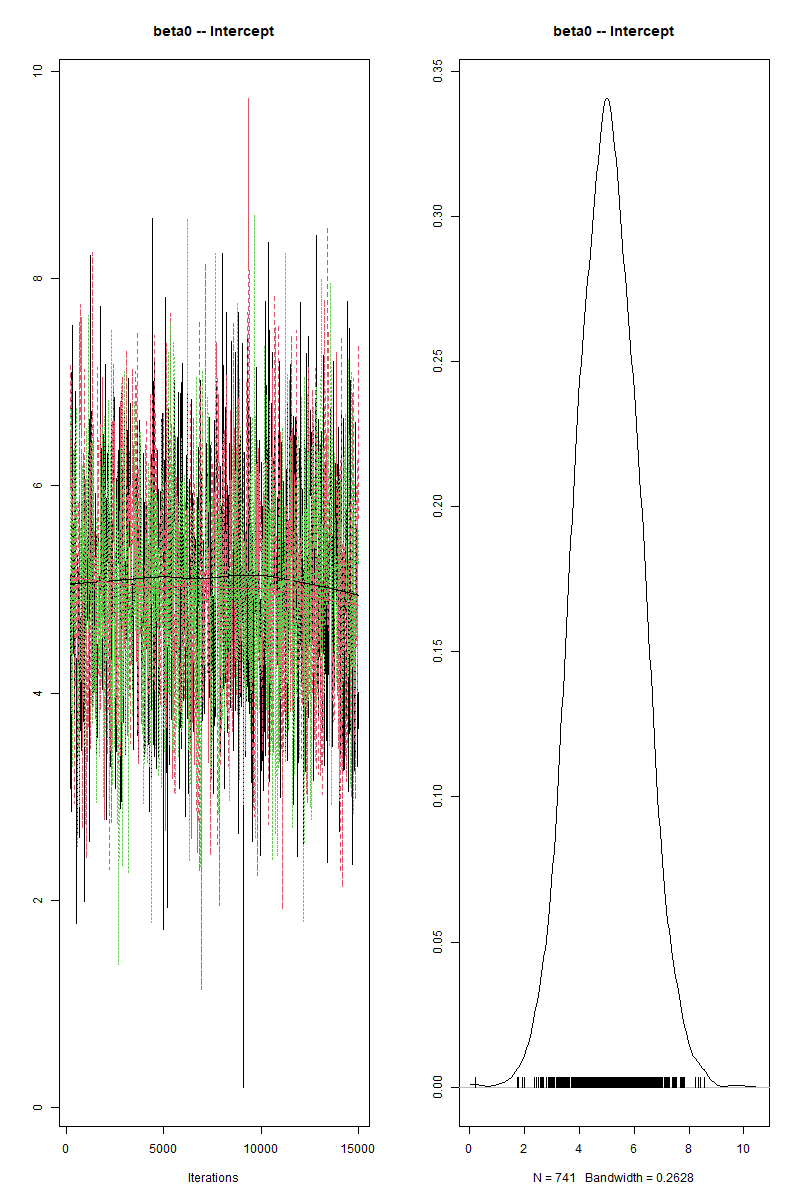
\includegraphics[width=0.7\linewidth]{img/img-trace-beta0}
	\caption{Trace and posterior density plots for the parameter $\beta_0$ (Intercept). The trace plot shows samples from three chains with good mixing and no signs of divergence or drift. All chains fluctuate around a common central value and remain tightly overlapped throughout the sampling period, a sign of stable convergence. The density plot shows a unimodal posterior distribution, peaking near 5.0 and spanning a broad range from approximately 2 to 8. The shape of the curve is slightly asymmetric near the peak, but remains smooth overall. The rug plot confirms dense and well-distributed sampling, supporting a reliable estimate of the intercept parameter. This indicates that the model has effectively identified a stable posterior distribution for $\beta_0$.}
	\end{figure}


\begin{figure}[H]
	\centering
	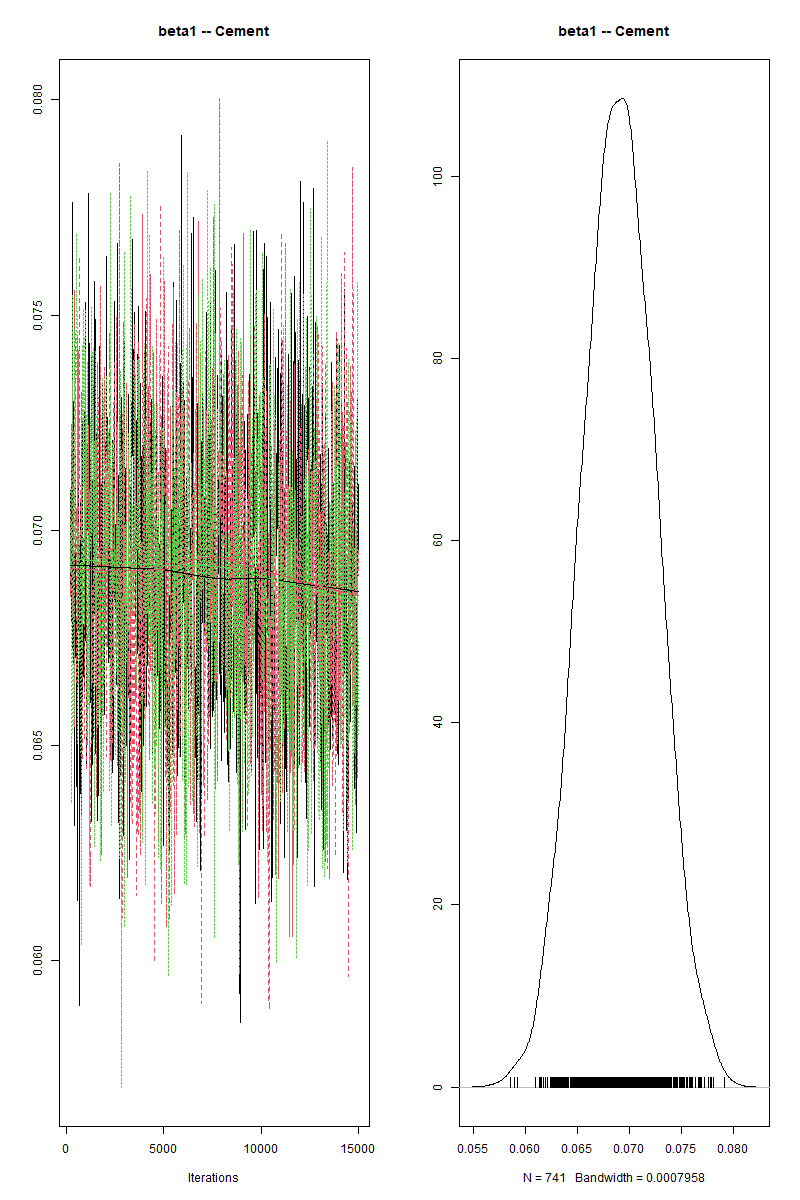
\includegraphics[width=0.7\linewidth]{img/img-trace-beta1}
	\caption{Trace and posterior density plots for the parameter $\beta_1$ (Cement). The trace plot on the left displays samples from three Markov Chain Monte Carlo (MCMC) chains. These chains show good mixing, with overlapping fluctuations around a stable mean after a burn-in period of 200 iterations. There is no visible drift or separation between the chains, and each chain explores the same region of the parameter space, indicating that convergence for $\beta_1$ has been achieved. The density plot on the right illustrates a smooth, unimodal posterior distribution, with the majority of the probability mass concentrated between approximately 0.060 and 0.078, peaking near 0.069. This suggests a strong positive effect of cement on concrete compressive strength.}
	\label{fig:img-trace-beta1}
\end{figure}

\begin{figure}[H]
	\centering
	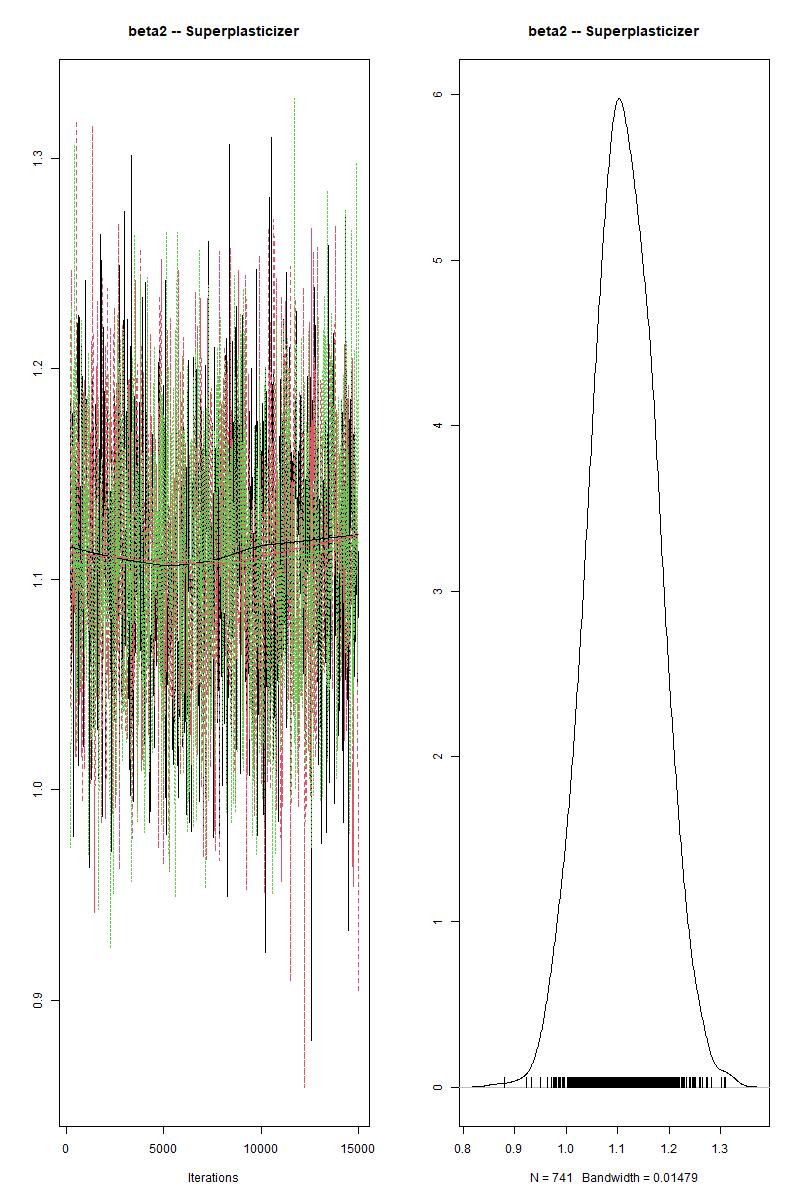
\includegraphics[width=0.7\linewidth]{img/img-trace-beta2}
	\caption{Trace and posterior density plots for the parameter $\beta_2$ (Superplasticizer). The trace plot shows three well-mixed chains with no indications of divergence, upward drift, or chain separation. The chains overlap consistently and fluctuate around a common mean, showing convergence and stationarity. The posterior density plot is unimodal, with the distribution between approximately 0.95 and 1.25, and a peak near 1.11. The curve is slightly asymmetric, with a marginally longer right tail, indicating slight skewness in the posterior. The rug plot confirms that sampling was dense and thorough across the high-probability region. These results indicate a stable and significant positive effect of superplasticizer on concrete compressive strength.}
	\label{fig:img-trace-beta2}
\end{figure}

\begin{figure}[H]
	\centering
	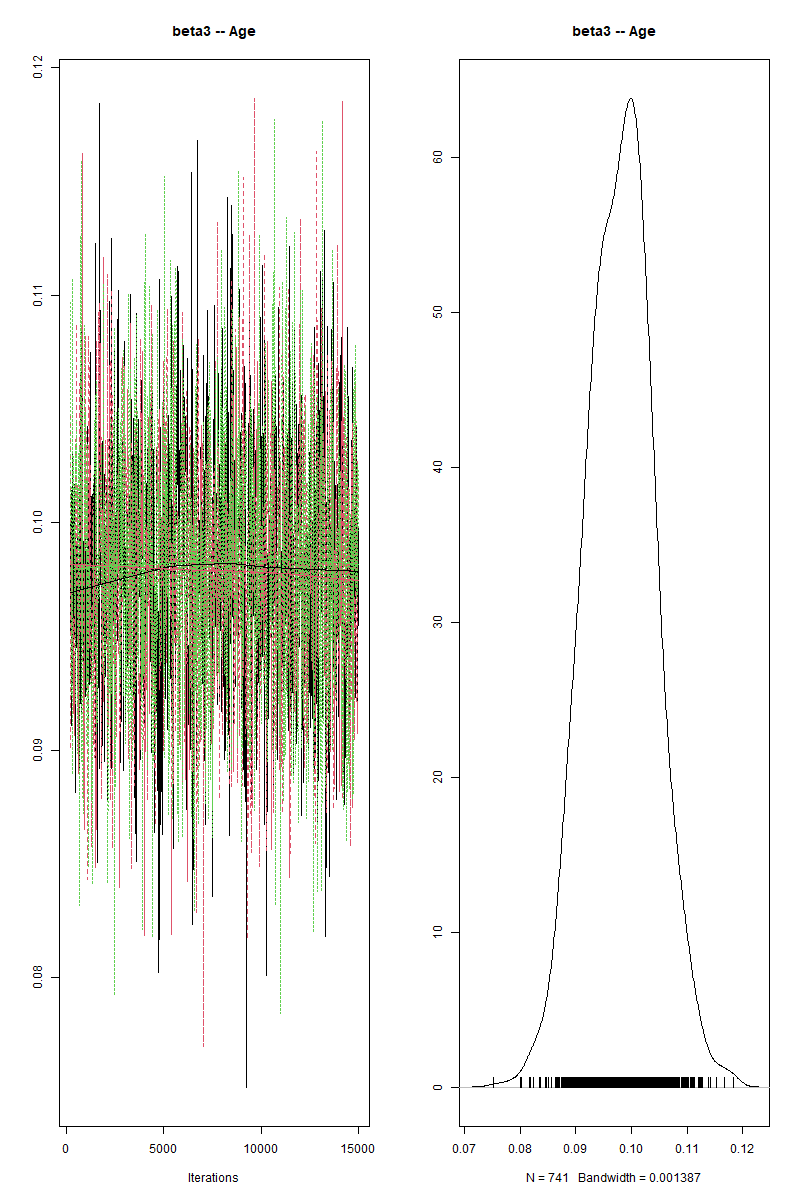
\includegraphics[width=0.7\linewidth]{img/img-trace-beta3}
	\caption{Trace and posterior density plots for the parameter $\beta_3$ (Age). The trace plot on the left displays three MCMC chains,exhibiting stable mixing  with consistent fluctuations around a common central value, thus indicating convergence. The density plot on the right shows a unimodal posterior distribution concentrated between approximately 0.085 and 0.110. While the distribution has a clearly defined peak near 0.098, a slight asymmetry is visible near the mode, with a more gradual slope on the right side, indicating mild skewness. The rug plot confirms a dense and even sampling of values, supporting a reliable and stable estimate for the effect of age on compressive strength.}
	\label{fig:img-trace-beta3}
\end{figure}

\begin{figure}[H]
	\centering
	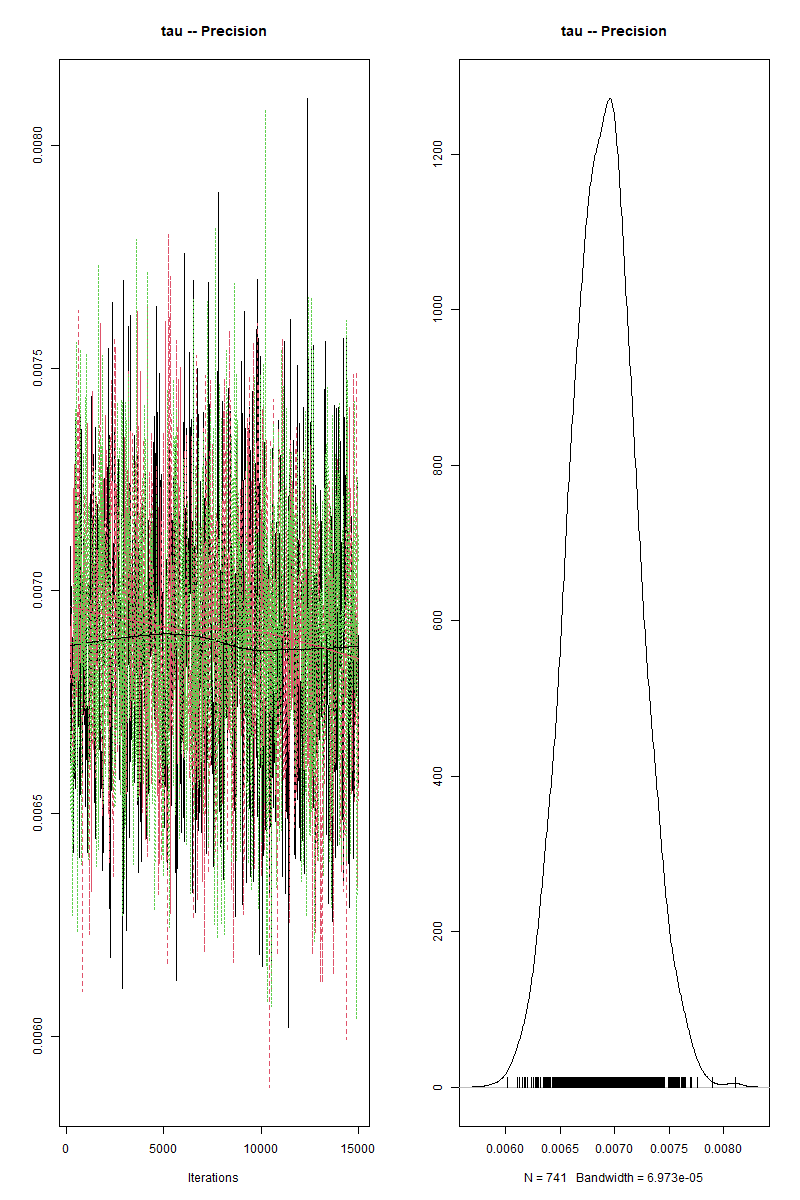
\includegraphics[width=0.7\linewidth]{img/img-trace-tao}
	\caption{Trace and posterior density plots for the parameter $\tau$ (precision of the normal likelihood). The trace plot shows good chain mixing and stationarity across all three chains, with no divergence, drift, or separation after burn-in. Fluctuations are consistently centred around a stable mean, showing convergence. The posterior density plot reveals a narrow and sharply peaked unimodal distribution concentrated between approximately 0.0063 and 0.0078, peaking near 0.0069, showing a tightly constrained estimate of the model’s residual precision. The rug plot below the density curve confirms dense and stable sampling from the posterior. This supports reliable inference for the precision parameter $\tau$.}
	\label{fig:img-trace-tao}
\end{figure}


\begin{figure}[H]
	\centering
	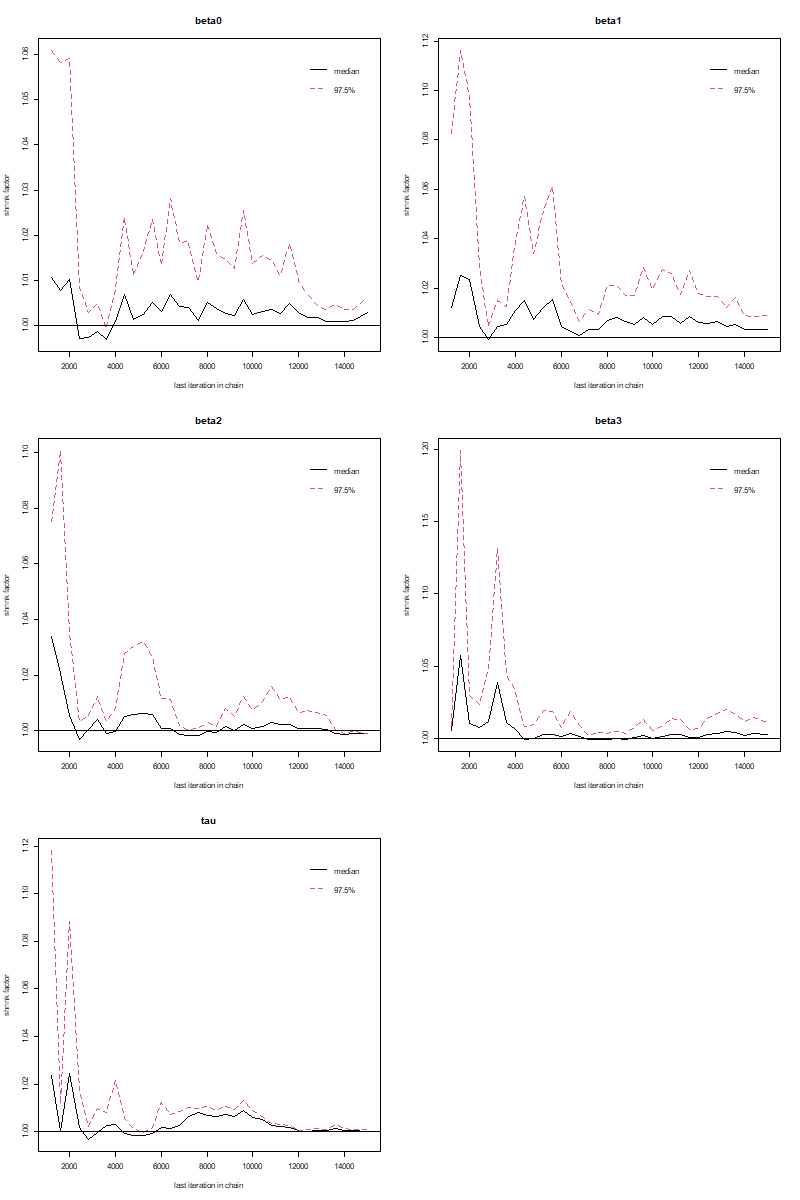
\includegraphics[width=0.7\linewidth]{img/img-gelman-plot-all}
	\caption{Gelman--Rubin diagnostic plots for all monitored parameters: intercept, cement, superplasticizer, age, and precision. The plots show the evolution of the shrink factor across increasing chain lengths. All parameters converge to Potential Scale Reduction Factor values close to 1.00 with their 97.5\% confidence intervals stabilising below 1.05. Convergence for all parameters appears to occur around iteration 6000, after which the shrink factors remain flat and close to unity. This shows that the chains for all parameters have likely converged to the same posterior distribution and that no substantial between-chain variation remains.}
	\label{fig:img-gelman-plot-all}
\end{figure}


\begin{figure}[H]
	\centering
	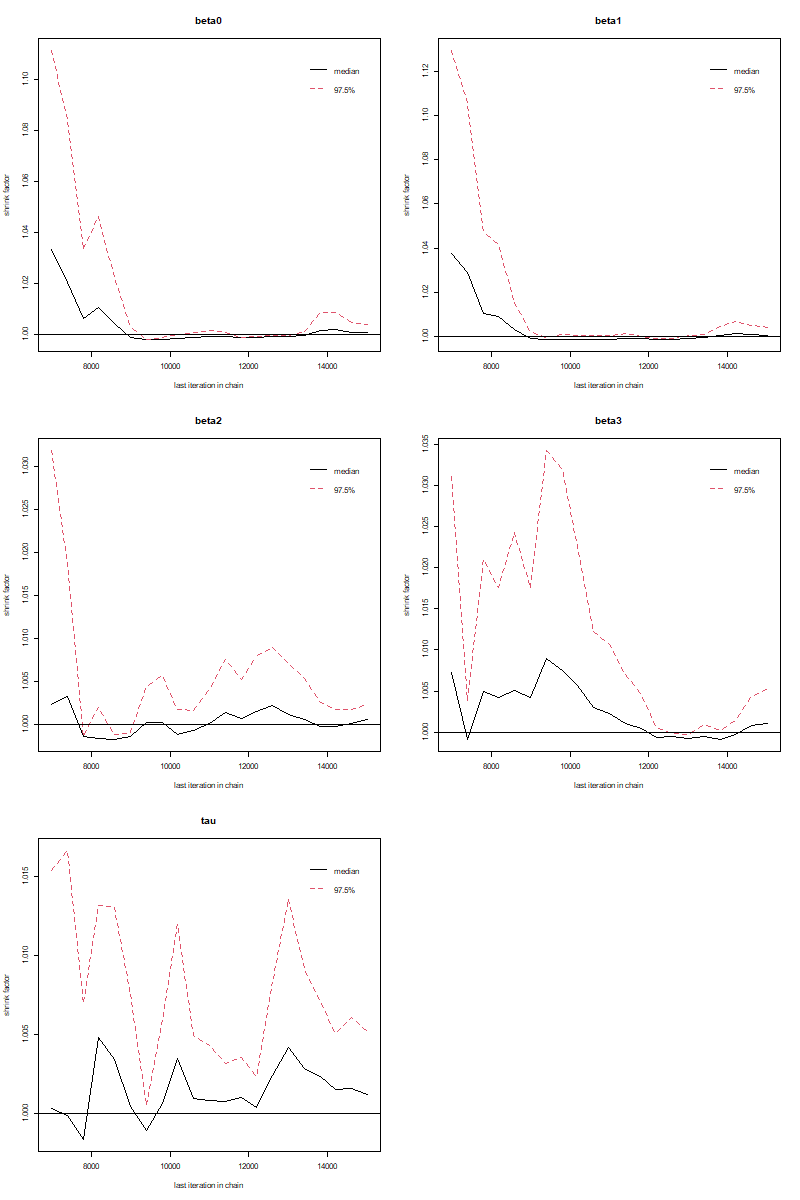
\includegraphics[width=0.7\linewidth]{img/img-gelman-plot-all-bi}
	\caption{Gelman-Rubin diagnostic plots for all monitored parameters following the removal of the first 6000 iterations as burn-in. After burn-in, all parameters show Potential Scale Reduction Factor values stabilising near 1.00, with their 97.5\% confidence intervals remaining below 1.05, indicating convergence. This confirms that discarding the initial 6000 iterations was effective in eliminating non-stationary behaviour, and that the retained samples are representative of the joint posterior distribution.}	\label{fig:img-gelman-plot-all-bi}
\end{figure}


The Gelman-Rubin Potential Scale Reduction Factor convergence diagnostic was also considered for accuracy. As shown in Figure all parameters have Potential Scale Reduction Factor point estimates equal to or very close to 1.00, with upper confidence limits not exceeding 1.03, confirming that the chains have mixed well and that the sampling process is stable and reliable for posterior inference.

\begin{figure}[H]
	\centering
	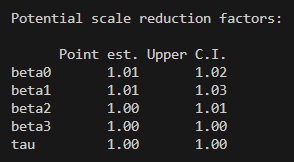
\includegraphics[width=0.7\linewidth]{img/img-psrf}
	\caption{Potential Scale Reduction Factor values for all monitored parameters. All point estimates are close to 1.00, and upper confidence intervals remain below the typically accepted threshold of 1.05, indicating convergence across chains for each parameter.}
	\label{fig:img-psrf}
\end{figure}


To assess the reliability and efficiency of the Markov Chain Monte Carlo sampling process, we examined two key accuracy diagnostics: effective sample size  and autocorrelation of the samples.

The effective sample sizes for all parameters were obtained using the summary() function on the Markov Chain Monte Carlo output object.

The effective sample size tells us how many of the samples from the Markov Chain Monte Carlo simulation are as useful as completely independent values. This is important because, in Markov Chain Monte Carlo, the samples are usually correlated, meaning each one is slightly influenced by the one before it. So, even if we run many iterations, the actual amount of "independent information" is lower.
In this analysis, each chain had about 451 effective samples for each parameter after discarding the burn-in and applying thinning (keeping every 20th sample). Since we ran three chains, that means we had over 1300 effective samples per parameter, meaning that the Markov Chain Monte Carlo sampling worked well and gave us enough reliable information to make accurate conclusions from the posterior distributions.

The time-series standard errors were small for all parameters (e.g., $\beta_0$: 0.030, $\beta_1$: 0.000098, $\beta_2$: 0.00164), confirming high sampling precision and low Monte Carlo error. These diagnostics collectively indicate that the model's parameter estimates are stable, reliable, and based on an efficient sampling process.


\begin{figure}[H]
	\centering
	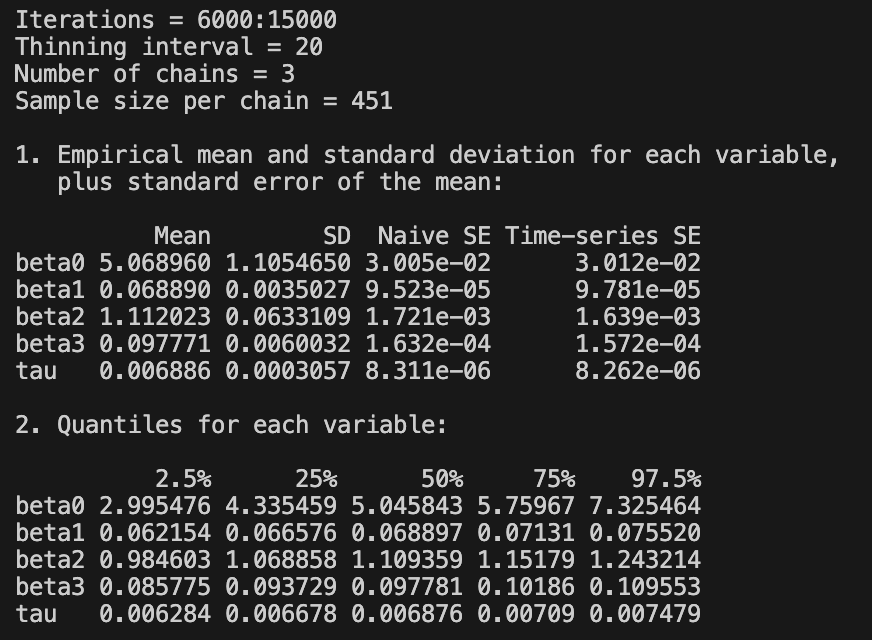
\includegraphics[width=0.7\linewidth]{img/img-summary}
	\caption{Summary statistics for all model parameters after burn-in and thinning.}	
	\label{fig:img-summary}
\end{figure}


Autocorrelation plots are used to assess how much each sample in a Markov Chain Monte Carlo simulation depends on the samples that came before it. In a well-mixed Markov Chain Monte Carlo chain, we expect the correlation between successive samples to decline rapidly as the lag increases; that is, samples become effectively independent as we move further apart along the chain. In an autocorrelation plot, each vertical bar represents the correlation at a particular lag. A plot showing high autocorrelation across many lags indicates poor mixing and slow convergence, while a plot where autocorrelation drops quickly to near zero suggests good mixing and efficient sampling. Ideally, the autocorrelation should be close to zero after just a few lags, indicating that the chain is exploring the posterior distribution effectively and that the resulting samples are reliable for inference.


\begin{figure}[H]
	\centering
	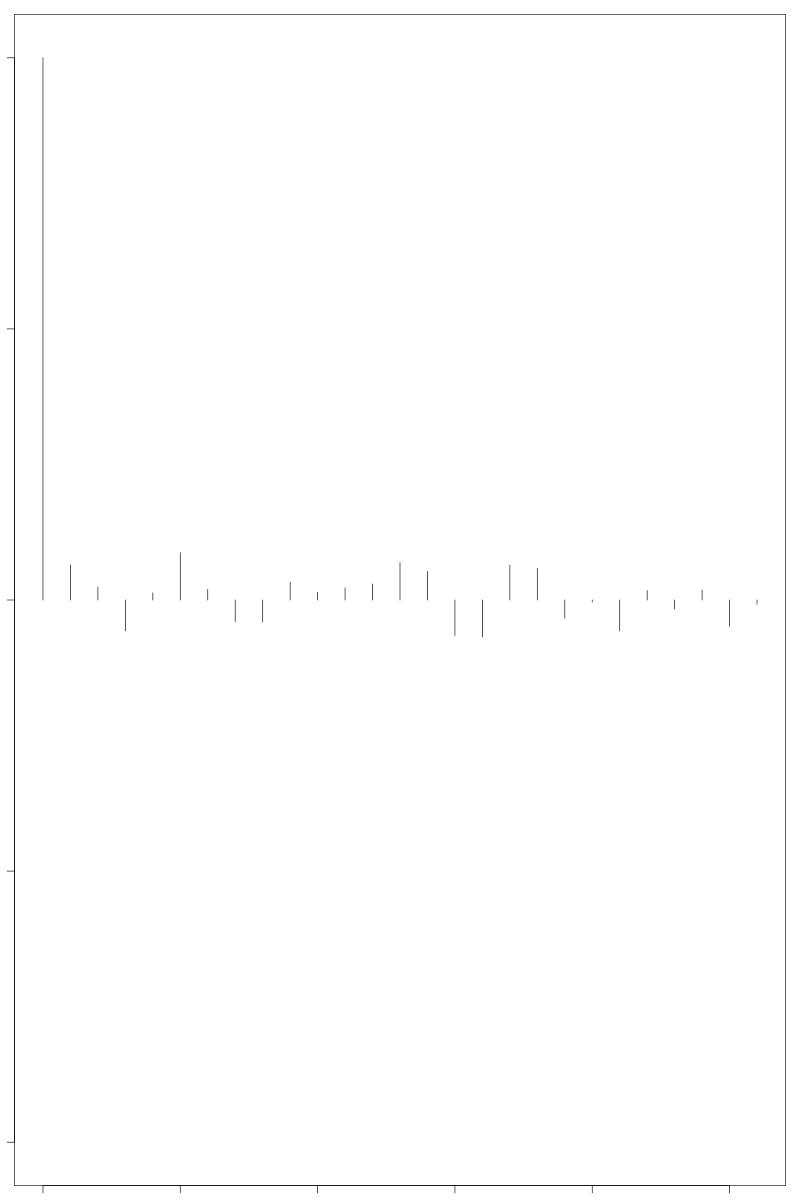
\includegraphics[width=0.7\linewidth]{img/img-autocorr-beta0}
	\caption{Autocorrelation plot for MCMC samples of $\beta_0$. The plot shows a rapid decline in autocorrelation after lag 1, with subsequent lags fluctuating closely around zero. This pattern indicates  minimal serial correlation and suggests that the chain for $\beta_0$ mixes well, resulting in effectively independent samples suitable for posterior inference.}
	\label{fig:img-autocorr-beta0}
\end{figure}


\begin{figure}
	\centering
	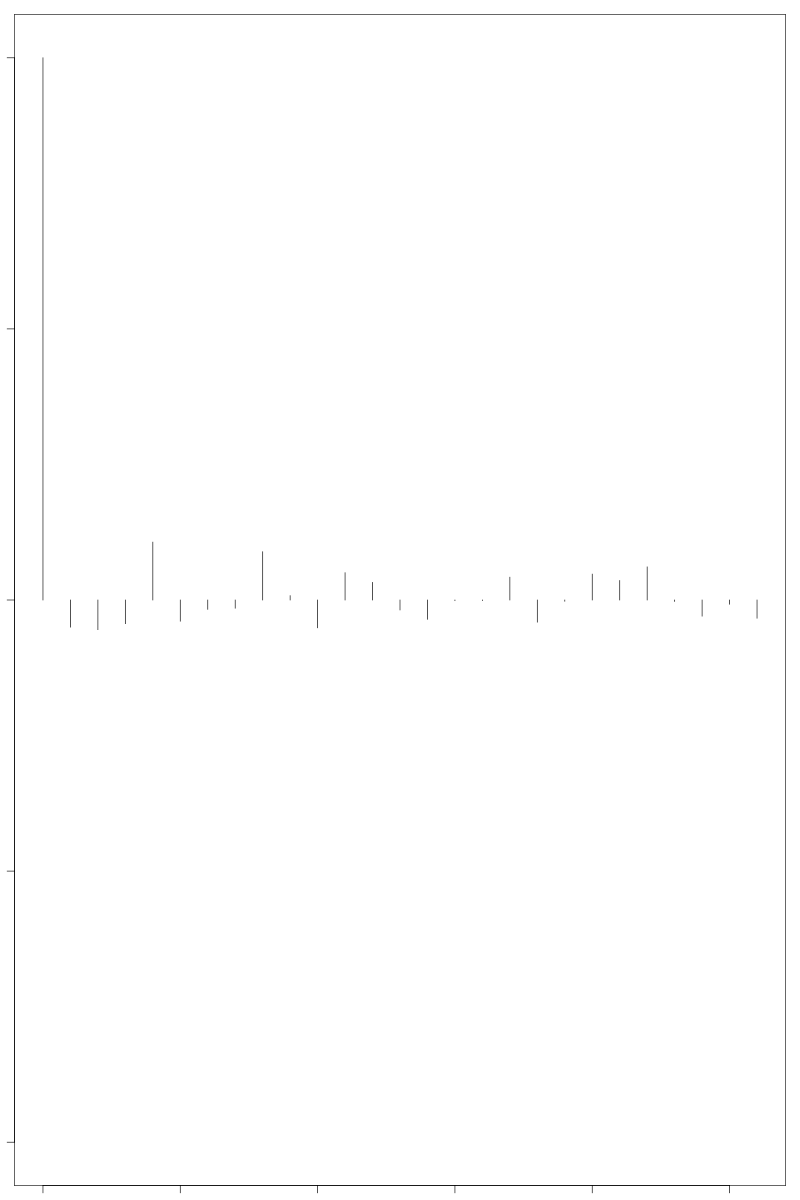
\includegraphics[width=0.7\linewidth]{img/img-autocorr-beta1}
	\caption{Autocorrelation plot for MCMC samples of $\beta_1$. As with $\beta_0$, the autocorrelation drops steeply after the first lag and remains near zero thereafter, confirming low intra-chain dependence and high sampling efficiency, implying that the posterior samples for $\beta_1$ are reliable and representative of the target distribution.}
	\label{fig:img-autocorr-beta1}
\end{figure}

\begin{figure}
	\centering
	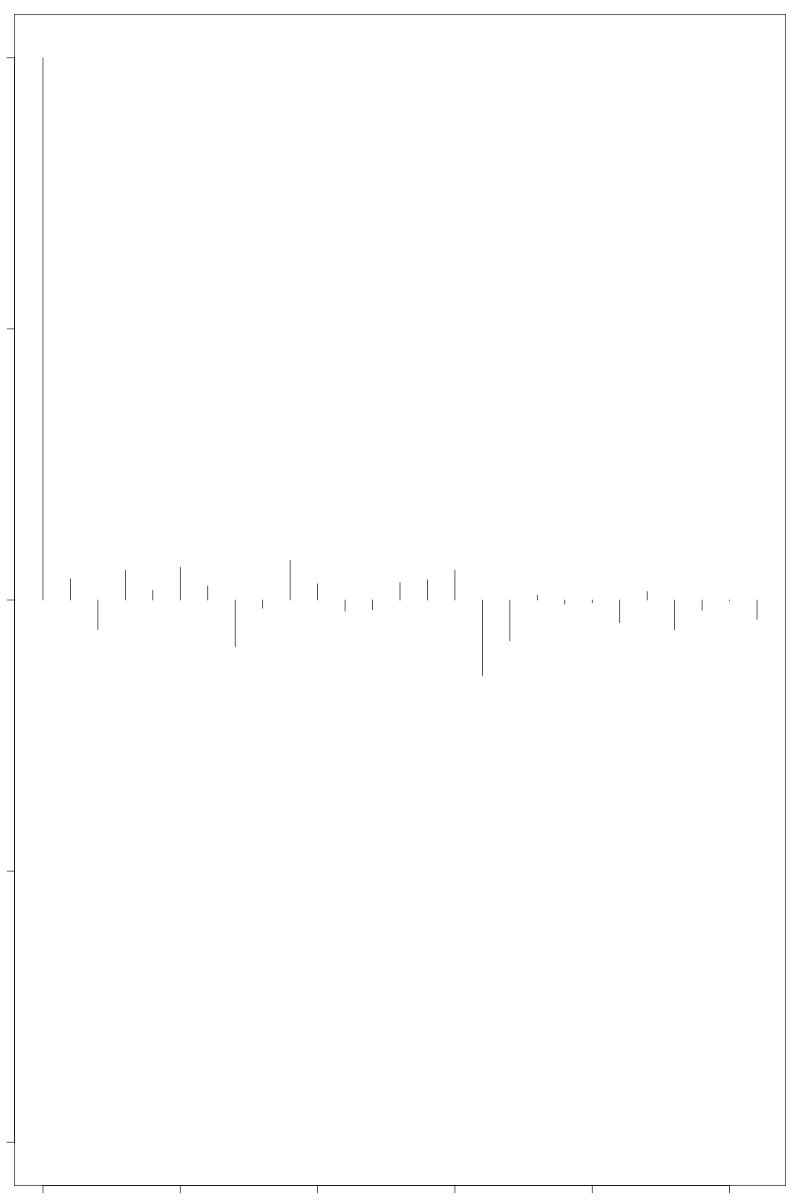
\includegraphics[width=0.7\linewidth]{img/img-autocorr-beta2}
	\caption{Autocorrelation plot for MCMC samples of $\beta_2$. The autocorrelation declines sharply after lag 1 and quickly levels off near zero for subsequent lags. This pattern indicates low dependence between successive samples and effective mixing of the chain, supporting the reliability of the posterior estimates for $\beta_2$.}
	\label{fig:img-autocorr-beta2}
\end{figure}

\begin{figure}
	\centering
	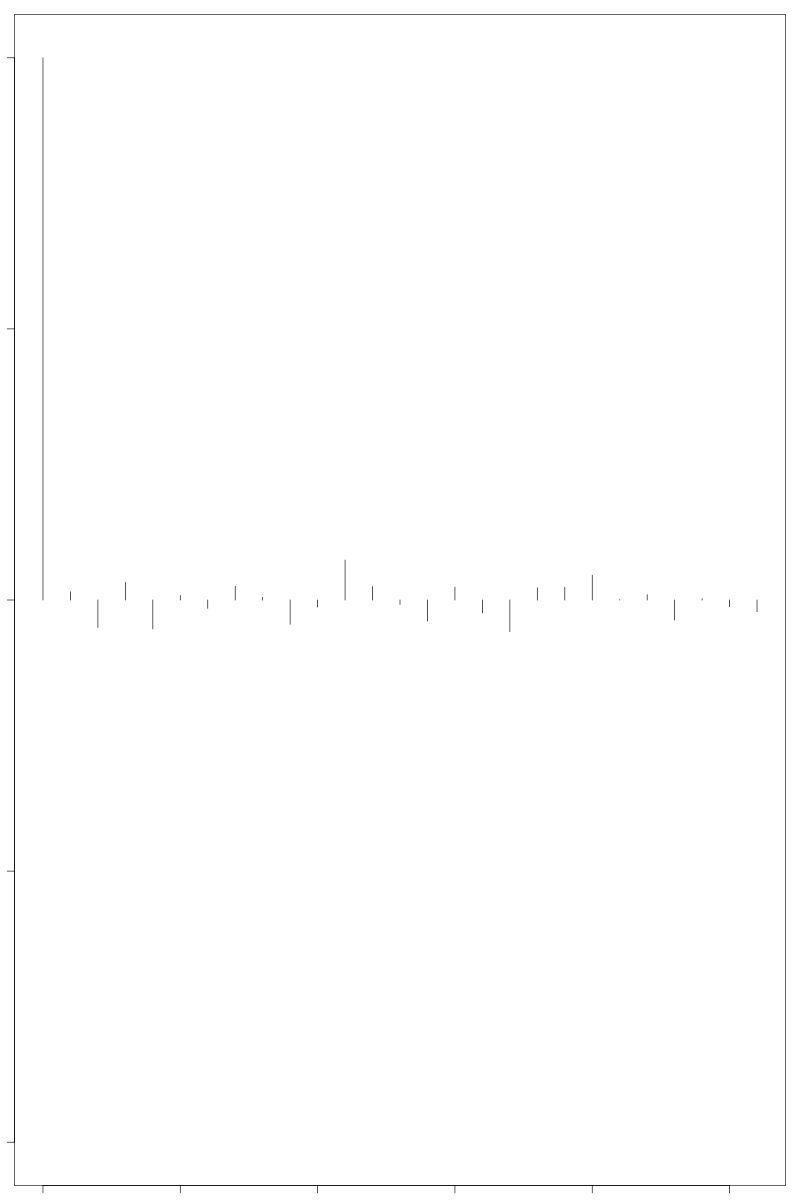
\includegraphics[width=0.7\linewidth]{img/img-autocorr-beta3}
	\caption{Autocorrelation plot for MCMC samples of $\beta_3$. The autocorrelation rapidly decays after lag 1 and remains close to zero for all subsequent lags, indicating minimal correlation between samples. This suggests that the MCMC chains for $\beta_3$ are mixing efficiently and producing effectively independent samples.}
	\label{fig:img-autocorr-beta3}
\end{figure}

\begin{figure}
	\centering
	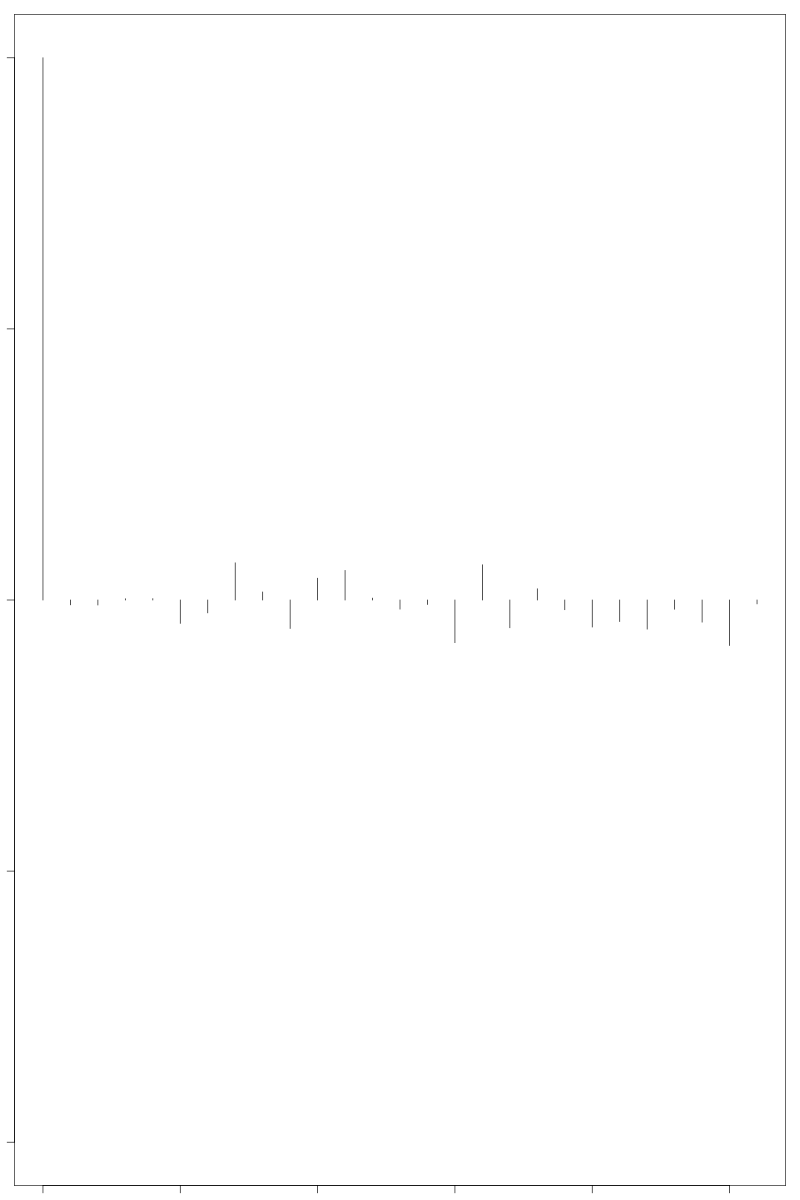
\includegraphics[width=0.7\linewidth]{img/img-autocorr-tao}
	\caption{Autocorrelation plot for MCMC samples of $\tau$ (precision parameter). The autocorrelation drops steeply after lag 1 and fluctuates around zero for all subsequent lags, suggesting low serial correlation. This indicates that the MCMC sampler produced nearly independent draws, supporting efficient posterior estimation for the precision.}
	\label{fig:img-autocorr-tao}
\end{figure}



\subsection{A discussion of the posterior distributions obtained from the analysis based on the
plots and summary statistics (which need to be presented in the text). Discuss also
how the posterior distributions of the model parameters can be used to predict new
values of the response variable Y, given only values for the explanatory variables
are available (prediction problem). Include both the interpretation of the parameter
uncertainty and how it propagates into predictions for new observations.}



The Bayesian linear regression model produced posterior distributions for all parameters; the intercept $\beta_0$, and the coefficients for cement ($\beta_1$), superplasticizer ($\beta_2$), and age ($\beta_3$), along with the residual precision parameter $\tau$. The posterior summaries indicate how each predictor is associated with the concrete compressive strength after accounting for uncertainty and prior beliefs.

Table~\ref{tab:posterior_summary} presents the posterior mean, standard deviation, and the 95\% credible interval for each parameter. None of the 95\% credible intervals include 0, which suggests that all predictors have a statistically meaningful association with the response variable. The posterior distributions reveal meaningful associations between the predictors and the response variable. The cement coefficient ($\beta_1$) has a positive mean effect with a narrow credible interval, indicating a consistent and stable contribution of cement to compressive strength. The effect of superplasticizer ($\beta_2$) remains the most prominent, with its posterior centred substantially away from zero, suggesting a strong and reliably positive influence. The age coefficient ($\beta_3$) is modest but tightly concentrated, implying that even small increases in curing time yield measurable improvements in strength. The intercept term ($\beta_0$) exhibits greater variability, reflecting the model's baseline uncertainty when predictors are near zero. Finally, the residual precision parameter ($\tau$) results in a relatively narrow distribution, indicating a well-estimated error structure and providing confidence in the model's predictive consistency. Collectively, these posterior characteristics reinforce the significance of each predictor while quantifying their uncertainty, supporting robust and interpretable inference.

\begin{table}[H]
	\centering
	\begin{tabular}{|l|r|r|c|}
		\hline
		\textbf{Parameter} & \textbf{Posterior Mean} & \textbf{SD} & \textbf{95\% Credible Interval} \\
		\hline
		$\beta_0$ (Intercept)         & 5.069 & 1.105 & [2.995, 7.325] \\
		$\beta_1$ (Cement)            & 0.0689 & 0.0035 & [0.062, 0.076] \\
		$\beta_2$ (Superplasticizer)  & 1.112 & 0.063 & [0.984, 1.243] \\
		$\beta_3$ (Age)               & 0.0980 & 0.0061 & [0.086, 0.110] \\
		$\tau$ (Precision)            & 0.00689 & 0.00031 & [0.00628, 0.00750] \\
		\hline
	\end{tabular}
	\caption{Posterior means, standard deviations, and 95\% credible intervals.}
	\label{tab:posterior_summary}
\end{table}


The following code was implemented to predict new values of the response variable:

\begin{lstlisting}

#extract post samples -- generate a bunch of samples for each posterior distribution
samples_matrix <- as.matrix(post_burned)

#new values --
x_new <- c(300, 8, 28)

#compute mu for each -- scale the samples with the example values
mu_pred <- samples_matrix[, "beta0"] +
samples_matrix[, "beta1"] * x_new[1] +
samples_matrix[, "beta2"] * x_new[2] +
samples_matrix[, "beta3"] * x_new[3]

#distrib of pred mean --> distr of outcomes by adding resdl noise
tau_samples <- samples_matrix[, "tau"]
y_pred <- rnorm(length(mu_pred), mean = mu_pred, sd = 1 / sqrt(tau_samples))

print("Summary of prediction")
print(summary(y_pred))
print(quantile(y_pred, c(0.025, 0.5, 0.975)))


df <- data.frame(
predictive = y_pred,
expected = mu_pred
)


plt <- ggplot(df, aes(x = predictive)) +
geom_density(fill = "skyblue", alpha = 0.5) +
geom_vline(aes(xintercept = mean(predictive)), color = "blue", linetype = "dashed") +
geom_vline(aes(xintercept = quantile(predictive, 0.025)), linetype = "dotted") +
geom_vline(aes(xintercept = quantile(predictive, 0.975)), linetype = "dotted") +
labs(title = "Posterior Predictive Distribution",
x = "Predicted Strength (MPa)", y = "Density") +
theme_minimal()
plot(plt)
\end{lstlisting}


\begin{itemize}
	\item To predict the compressive strength of a new concrete mix, the posterior distributions of the regression coefficients obtained from Markov Chain Monte Carlo sampling were used.
	
	\item Values for example predictor variables were specified (cement = 300, superplasticizer = 8, age = 28).
	
	\item For each posterior sample, a predicted linear mean $\mu_{\text{pred}}$ was computed using:
	$$
	\mu_{\text{pred}} = \beta_0 + \beta_1 x_{\text{cement}} + \beta_2 x_{\text{superplasticizer}} + \beta_3 x_{\text{age}}
	$$
	
	\item Using $\mu_{\text{pred}}$, the corresponding predicted value $y_{\text{pred}}$ was then drawn from a normal distribution:
	$$
	y_{\text{pred}} \sim \mathcal{N}(\mu_{\text{pred}}, \tau^{-1})
	$$
	where $\tau$ is the posterior precision from each sample.
	\item This procedure accounts for both parameter uncertainty and residual noise in generating predictive values.
	\item A summary of the predictive distribution, including mean and 95\% credible interval, was computed and visualised.
\end{itemize}


Figure \ref{fig:img-post-mean-pred} shows the distributions of the expected mean response and posterior prediction. ThFigure \ref{fig:img-post-mean-pred} illustrates the distributions of the expected mean response and posterior predictions. The expected mean response is tightly concentrated, reflecting certainty around the average response. In contrast, the predictive distribution is flatter due to noise in the observations.e former is, as expected, tightly concentrated, thus reflecting certainty around the average response. The predictive distribution is flatter due to noise in the observations.

\begin{figure}[H]
	\centering
	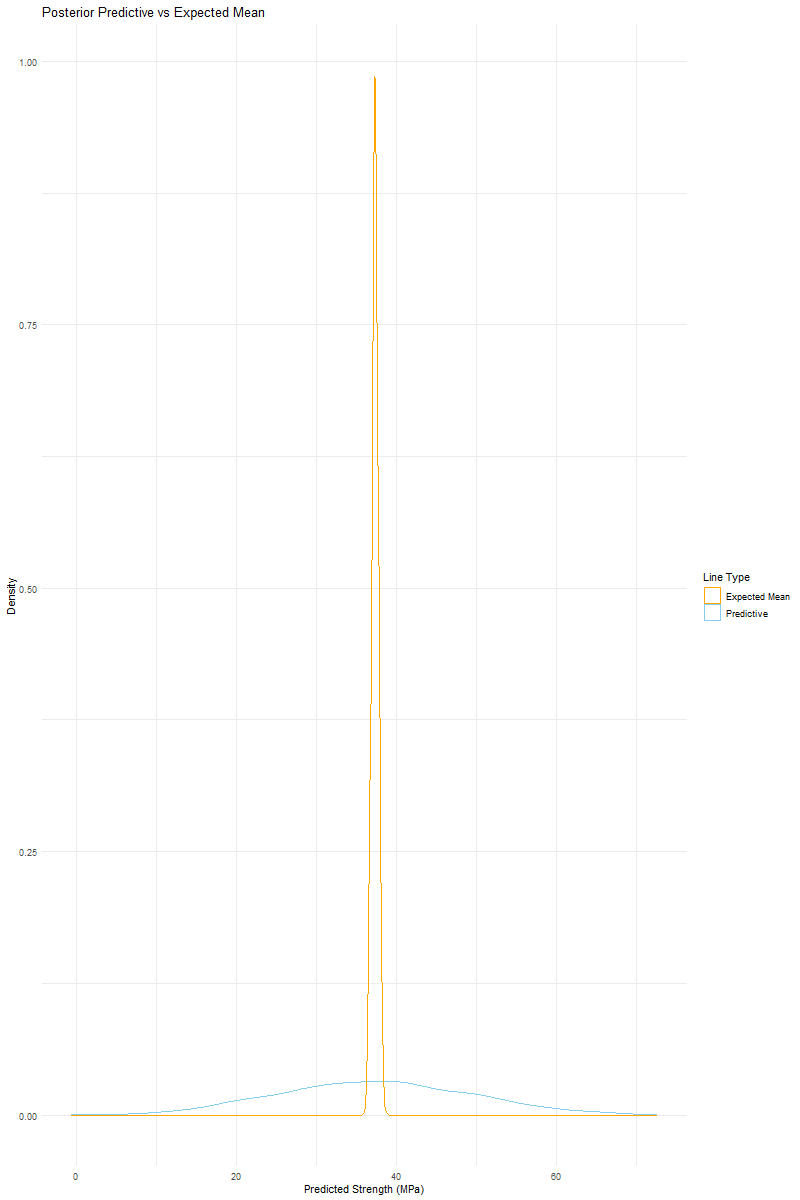
\includegraphics[width=0.7\linewidth]{img/img-post-mean-pred}
	\caption{Comparison between the posterior predictive distribution and the distribution of the expected mean response. The narrow orange curve represents the distribution of the predicted mean response $\mu$ based on posterior samples of the model parameters. The wider blue curve shows the posterior predictive distribution for new observations, which incorporates both parameter uncertainty and residual noise. The increased spread in the predictive distribution reflects the variability expected in real-world observations.}
	\label{fig:img-post-mean-pred}
\end{figure}

\subsection{Also present the R script, including comments that explain what each section does in
an appendix. }

\begin{itemize}
	\item The code is available in the following GitHub repository: \\ \texttt{https://github.com/carmelgafa/sci5020.}
	\item It was developed using Visual Studio Code alongside the VSCode R extension. Some minor precautions, such as printing to a variable, were necessary during development.
	\item The code was tested using R version 4.4.2.
	\item The code can be found in Appendix \ref{appendix:a}
\end{itemize}



	
\section{Question 2}

Let $ \textbf{x} = (x_1, \dots, x_n)'$ be a set of observations. Consider the following Bayesian model:

$$
p(\mu, \sigma^2 \mid \textbf{x}) 
\propto 
\left[ \prod_{i=1}^n \mathcal{N}(x_i \mid \mu, \sigma^2) \right] 
\mathcal{N}(\mu \mid m_0, v_0^2) 
\Gamma(\tau \mid a, b), 
\quad \tau = \sigma^{-2}
$$

We do not know explicitly the posterior here but we know through the theory of conjugate priors that:

$$
p(\mu \mid \textbf{x}, \sigma^2) 
\propto 
\left[ \prod_{i=1}^n \mathcal{N}(x_i \mid \mu, \sigma^2) \right] 
\mathcal{N}(\mu \mid m_0, v_0^2) = 
\mathcal{N} \left( \frac{n \bar{x} + v_0^{-2} m_0}{n + v_0^{-2}}, \left(n + v_0^{-2} \right)^{-1} \right)
$$

$$
p(\tau \mid \textbf{x}, \sigma^2) 
\propto 
\left[ \prod_{i=1}^n \mathcal{N}(x_i \mid \mu, \sigma^2) \right] 
\Gamma(\tau \mid a, b) = \Gamma\left( a + \frac{n}{2}, \frac{1}{2} \sum_{i=1}^n (x_i - \mu)^2 + b \right)
$$


\noindent \textbf{Recap of problem statement:}\\

Let $\mathbf{x} = (x_1, x_2, \dots, x_n)'$ be defined as a vector of observed data points. A Bayesian model is considered, in which the data are assumed to be generated from a Normal distribution with an unknown mean $\mu$ and unknown variance $\sigma^2$:
$$
x_i \mid \mu, \sigma^2 \sim \mathcal{N}(\mu, \sigma^2), \quad i = 1, \dots, n
$$

A Bayesian approach is adopted, and prior distributions are specified for the unknown parameters $\mu$ and $\sigma^2$. Specifically, a Normal prior is placed on the mean $\mu$, and a Gamma prior is assigned to the precision $\tau = \sigma^{-2}$:
$$
\mu \mid \tau \sim \mathcal{N}(m_0, v_0^2), \quad \tau \sim \text{Gamma}(a, b)
$$

In this hierarchical Bayesian model, a Normal prior is assigned to the mean $\mu$ conditional on the precision $\tau$, and a Gamma prior is placed on $\tau$. This results in the following joint prior:
$$
p(\mu, \tau) = p(\mu \mid \tau) \cdot p(\tau)
$$

By using conjugate priors, it is ensured that the posterior distributions for $\mu$ and $\tau$ remain in standard, tractable forms (Normal and Gamma), thereby facilitating efficient sampling through the Gibbs sampling method.

The complete joint posterior distribution $p(\mu, \tau \mid \mathbf{x})$ is not known in closed form. However, the theory of conjugate priors allows the full conditional distributions to be derived analytically:

\begin{itemize}
	\item The conditional posterior distribution of $\mu$ given $\tau$ and $\mathbf{x}$ is a Normal distribution:
	$$
	\mu \mid \mathbf{x}, \tau \sim \mathcal{N}\left( \frac{n \bar{x} + v_0^{-2} m_0}{n + v_0^{-2}}, \left(n + v_0^{-2} \right)^{-1} \right)
	$$
	\item The conditional posterior distribution of $\tau$ given $\mu$ and $\mathbf{x}$ is a Gamma distribution:
	$$
	\tau \mid \mathbf{x}, \mu \sim \text{Gamma} \left( a + \frac{n}{2}, \; b + \frac{1}{2} \sum_{i=1}^n (x_i - \mu)^2 \right)
	$$
\end{itemize}

\noindent These conditional distributions constitute the foundation of a Gibbs sampling algorithm, by which samples from the joint posterior can be obtained through iterative sampling.

The implementation of this Bayesian model is now undertaken through the following steps:

\begin{enumerate}
	\item[(i)] \textbf{Simulation of data.} Fixed values are selected for $\mu$ and $\sigma^2$, and 100 observations are drawn from a Normal distribution with the specified parameters:
	$$
	x_i \sim \mathcal{N}(\mu, \sigma^2), \quad i = 1, \ldots, 100
	$$
	
	\item[(ii)] \textbf{Specification of priors.} Hyperparameters $m_0$, $v_0^2$, $a$, and $b$ are chosen to reflect non-informative prior beliefs about $\mu$ and $\tau$. For instance:
	$$
	m_0 = 0, \quad v_0^2 = 10^6, \quad a = b = 0.01
	$$
	
	\item[(iii)] \textbf{Execution of Gibbs sampling.} An initial value $\tau^{(0)}$ is selected. Gibbs sampling is then used to generate 10{,}000 samples from the joint posterior of $\mu$ and $\tau$. At each iteration $t$, the following steps are performed:
	$$
	\mu^{(t)} \sim \mathcal{N}\left( \frac{n \bar{x} + v_0^{-2} m_0}{n + v_0^{-2}}, \left(\tau^{(t-1)}(n + v_0^{-2})\right)^{-1} \right)
	$$
	$$
	\tau^{(t)} \sim \text{Gamma} \left( a + \frac{n}{2}, \; b + \frac{1}{2} \sum_{i=1}^n (x_i - \mu^{(t)})^2 \right)
	$$
	A suitable number of initial samples are discarded as burn-in.
	
	\item[(iv)] \textbf{Assessment of convergence.} Diagnostic tools are used to evaluate whether the chains have converged and whether the burn-in period has been sufficient. In particular:
	\begin{itemize}
		\item A \texttt{traceplot} is produced for the sampled values of $\mu$ and $\tau$.
		\item The \texttt{autocorrelation function (ACF)} is examined to assess correlation between successive samples.
		\item The \texttt{effective sample size (ESS)} is computed to estimate the number of effectively independent draws.
	\end{itemize}
	These diagnostics are used to determine the adequacy of convergence and burn-in.
	
	\item[(v)] \textbf{Summarization of posterior distributions.} The \texttt{epdfPlot} function from the \texttt{EnvStats} package in R is employed to produce empirical posterior density estimates for $\mu$, $\tau$, and $\sigma^2 = \tau^{-1}$, using only post-burn-in samples.
\end{enumerate}



%The goal of Bayesian inference is to compute the posterior distribution of the parameters given the data:
%
%$$
%p(\mu, \tau \mid \mathbf{x}) \propto p(\mathbf{x} \mid \mu, \tau) \cdot p(\mu \mid \tau) \cdot p(\tau)
%$$
%
%The likelihood function for the independent normal observations is:
%
%$$
%p(\mathbf{x} \mid \mu, \tau) = \prod_{i=1}^n \left( \frac{\sqrt{\tau}}{\sqrt{2\pi}} \exp\left( -\frac{\tau}{2}(x_i - \mu)^2 \right) \right)
%$$
%
%Taking the product:
%
%$$
%p(\mathbf{x} \mid \mu, \tau) \propto \tau^{n/2} \exp\left( -\frac{\tau}{2} \sum_{i=1}^n (x_i - \mu)^2 \right)
%$$
%
%
%\[
%p(\mu \mid \tau) = \sqrt{\frac{\tau}{2\pi v_0^2}} \exp\left( -\frac{\tau}{2v_0^2} (\mu - m_0)^2 \right)
%\]
%
%The prior on $\tau$ is:
%
%$$
%p(\tau) \propto \tau^{a - 1} e^{-b\tau}
%$$
%
%Therefore, the joint posterior is:
%
%$$
%p(\mu, \tau \mid \mathbf{x}) \propto \tau^{n/2} \exp\left( -\frac{\tau}{2} \sum_{i=1}^n (x_i - \mu)^2 \right) \cdot \tau^{1/2} \exp\left( -\frac{\tau}{2v_0^2} (\mu - m_0)^2 \right) \cdot \tau^{a-1} e^{-b\tau}
%$$
%	
%Combining powers of $\tau$:
%
%$$
%p(\mu, \tau \mid \mathbf{x}) \propto \tau^{a + \frac{n+1}{2} - 1} \exp\left( -\tau \left[ \frac{1}{2} \sum_{i=1}^n (x_i - \mu)^2 + \frac{1}{2v_0^2} (\mu - m_0)^2 + b \right] \right)
%$$
%


\subsection{Decide on values for $\mu$ and $\sigma^2$ and simulate 100 values from a normal distribution with this mean and variance.}


\noindent \textbf{Part (i): Simulation of Data}

A dataset consisting of $n = 100$ observations was simulated from a normal distribution with mean $\mu = 5$ and variance $\sigma^2 = 4$. 

The resulting histogram of the simulated data confirms the approximate bell-shaped structure expected of normal distributions, centered around the mean.

The following code was used for simulation and visualization:

\begin{lstlisting}

## Question i

mu <- 5
sigma_2 <- 4
sigma <- sqrt(sigma_2)
n <- 100

set.seed(1001)
x <- rnorm(n, mean = mu, sd = sigma)

# Save histogram object (does not plot automatically)
plt <- hist(x, breaks = 50, col = "skyblue", main = "Histogram of Simulated Data",
xlab = "x values", border = "white", freq = FALSE)
plot(plt)

curve(dnorm(x, mean = mu, sd = sigma), col = "blue", lwd = 2, add = TRUE)
\end{lstlisting}



\begin{figure}[H]
	\centering
	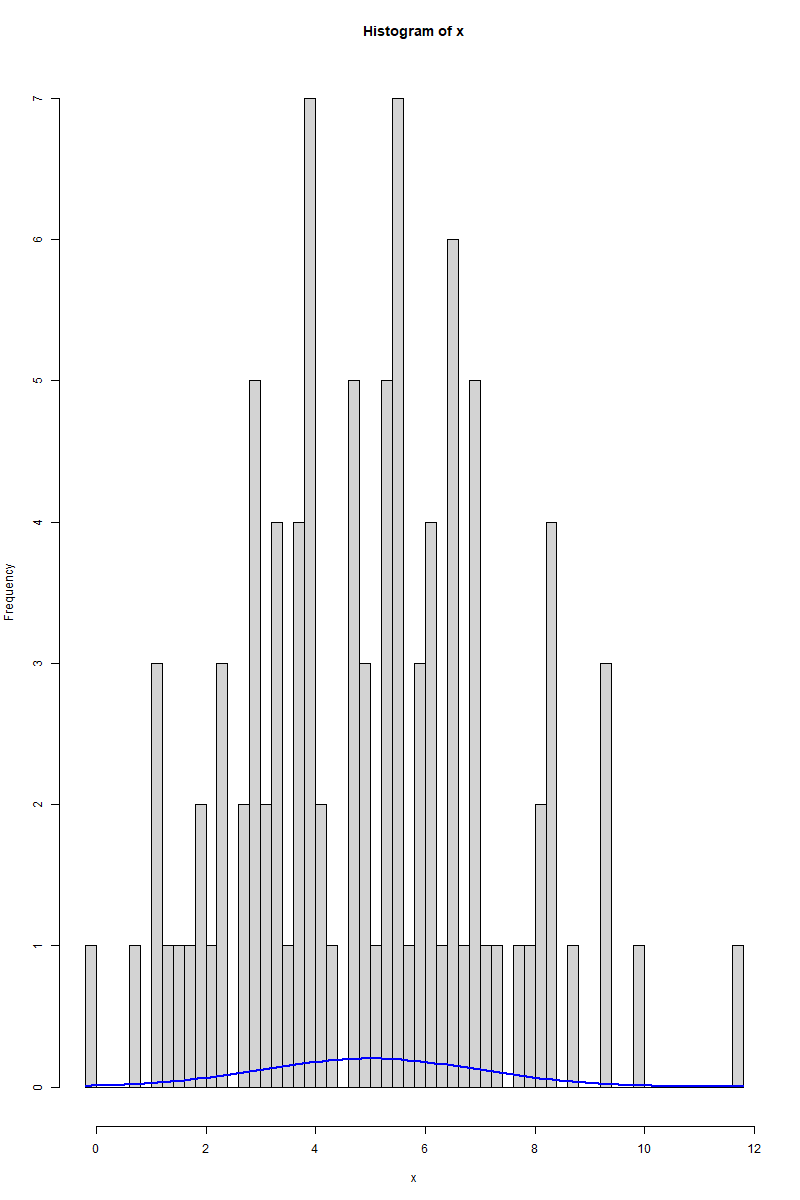
\includegraphics[width=0.7\linewidth]{img/img-2-norm-dist}
	\caption{Histogram of 100 simulated observations from a normal distribution with mean $\mu = 5$ and variance $\sigma^2 = 4$. The blue curve represents the theoretical density function of $\mathcal{N}(5, 2^2)$ superimposed on the histogram.}
	\label{fig:img-2-norm-dist}
\end{figure}


\subsection{Decide on hyperparameters $m_0, v_0^2, a, b$ which yield a non-informative prior.}


To use the Bayesian model, we need to define prior distributions for the unknown parameters $\mu$ and $\tau = \sigma^{-2}$. We will use a conjugate prior structure, which includes:

$$
\mu \mid \tau \sim \mathcal{N}(m_0, v_0^2), \quad \tau \sim \text{Gamma}(a, b)
$$

In this implementation, vague priors are used to show limited prior knowledge about the parameters. The following hyperparameter values are provided:

$$
m_0 = 0, \quad v_0^2 = 10^6, \quad a = 0.01, \quad b = 0.01
$$

This choice allows for a wide range of possible values for $\mu$, giving more weight to the data when making inferences. The Gamma prior on $\tau$ has a small shape and rate, creating a flat and broad distribution over all positive real numbers.

\noindent These prior choices ensure that the posterior distributions remain proper while contributing little information relative to the likelihood. This is a common strategy when the objective is to let the data primarily inform the inference.

\begin{lstlisting}
m0 <- 0
v0_sq <- 1e6
a <- 0.01
b <- 0.01
\end{lstlisting}




\subsection{Pick an initial value of $\tau$. Use Gibbs' sampling to simulate 10000 values of $\mu$ and $\tau$ (excluding an appropriately chosen burn-in period).}


With the conditional posterior distributions derived analytically, a Gibbs sampling algorithm is implemented to simulate from the joint posterior of $(\mu, \tau)$. The full conditionals are:

\begin{align*}
	\mu \mid \mathbf{x}, \tau &\sim \mathcal{N} \left( \frac{n \bar{x} + v_0^{-2} m_0}{n + v_0^{-2}}, \; \left( \tau(n + v_0^{-2}) \right)^{-1} \right) \\
	\tau \mid \mathbf{x}, \mu &\sim \text{Gamma} \left( a + \frac{n}{2}, \; b + \frac{1}{2} \sum_{i=1}^n (x_i - \mu)^2 \right)
\end{align*}


The Gibbs sampler iteratively draws samples from the full conditional distributions of $\mu$ and $\tau$, constructing a Markov chain that converges to the joint posterior $p(\mu, \tau \mid \mathbf{x})$. The procedure is implemented as follows:

\begin{itemize}
	\item \textbf{Initialization}
	\begin{itemize}
		\item Set the number of iterations $T$ (10,000 in this case) and burn-in length (2000).
		\item Create storage vectors for sampled values of $\mu$ and $\tau$.
		\item Choose an initial value for $\tau^{(0)}$, e.g., the reciprocal of the sample variance.
	\end{itemize}
	
	\item \textbf{Repeat for each iteration $t = 1, \dots, T$:}
	\begin{enumerate}
		\item \textbf{Sample $\mu^{(t)} \mid \tau^{(t-1)}, \mathbf{x}$:}
		\begin{itemize}
			\item Compute the conditional posterior variance:
			$$
			\text{Var}(\mu \mid \cdot) = \left( \tau^{(t-1)} n + \frac{1}{v_0^2} \right)^{-1}
			$$
			\item Compute the conditional posterior mean:
			$$
			\text{Mean}(\mu \mid \cdot) = \text{Var}(\mu \mid \cdot) \cdot \left( \tau^{(t-1)} n \bar{x} + \frac{m_0}{v_0^2} \right)
			$$
			\item Draw $\mu^{(t)}$ from $\mathcal{N}(\text{Mean}, \text{Var})$.
		\end{itemize}
		
		\item \textbf{Sample $\tau^{(t)} \mid \mu^{(t)}, \mathbf{x}$:}
		\begin{itemize}
			\item Compute the shape parameter:
			$$
			a + \frac{n}{2}
			$$
			\item Compute the rate parameter:
			$$
			b + \frac{1}{2} \sum_{i=1}^n (x_i - \mu^{(t)})^2
			$$
			\item Draw $\tau^{(t)}$ from $\text{Gamma}(\text{shape}, \text{rate})$.
		\end{itemize}
		
		\item \textbf{Store the draws:}
		\begin{itemize}
			\item Save $\mu^{(t)}$ and $\tau^{(t)}$ to their respective storage vectors.
		\end{itemize}
	\end{enumerate}
	
	\item \textbf{Post-sampling:}
	\begin{itemize}
		\item Discard the first $2{,}000$ iterations as burn-in to mitigate the effect of the initial values.
		\item Use the remaining samples for inference and convergence diagnostics.
	\end{itemize}
\end{itemize}

Code used for this question:

\begin{lstlisting}
## Question iii

#sampler setting
n_iter <- 10000
burn_in <- 2000

#storeage for mu and tao 
mu_samples <- numeric(n_iter)
tau_samples <- numeric(n_iter)

#init tao
tau_current <- 1 / var(x)  # start with reasonable value

x_bar <- mean(x)

for (t in 1:n_iter) {
	var_mu <- 1 / (tau_current * n + 1 / v0_sq)
	mean_mu <- var_mu * (tau_current * n * x_bar + m0 / v0_sq)
	mu_current <- rnorm(1, mean = mean_mu, sd = sqrt(var_mu))
	
	#sample tao given mu
	shape_tau <- a + n / 2
	rate_tau <- b + sum((x - mu_current)^2) / 2
	tau_current <- rgamma(1, shape = shape_tau, rate = rate_tau)
	
	#store
	mu_samples[t] <- mu_current
	tau_samples[t] <- tau_current
}

#burn-in
mu_post <- mu_samples[(burn_in + 1):n_iter]
tau_post <- tau_samples[(burn_in + 1):n_iter]
sigma2_post <- 1 / tau_post  # for inference on variance


print(mean(mu_post))
print(quantile(mu_post, c(0.025, 0.5, 0.975)))
print(mean(sigma2_post))
print(quantile(sigma2_post, c(0.025, 0.5, 0.975)))
\end{lstlisting}


Figure \ref{fig:img-2-post-summary} shows the posterior summary obtained after burn-in was executed.


\begin{figure}
	\centering
	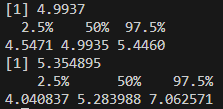
\includegraphics[width=0.7\linewidth]{img/img-2-post-summary}
	\caption{ Posterior summaries based on 8,000 post-burn-in samples from the Gibbs sampler. The estimated posterior mean of $\mu$ is approximately 4.99 with a 95\% credible interval of [4.55, 5.45]. The posterior mean of $\sigma^2$ is approximately 5.35 with a 95\% credible interval of [4.04, 7.06]. }
	\label{fig:img-2-post-summary}
\end{figure}

\begin{enumerate}
	\item The posterior estimate for $\mu$ is very close to the true value used in simulation: $\mu = 5$.

	\item The posterior estimate for $\sigma^2$ is slightly higher than the true value ($\sigma^2 = 4$), but it falls within the 95\% credible interval. This is expected given the relatively small sample size ($n = 100$). When the sample size was increased to $n = 1000$, the posterior estimate of $\sigma^2$ moved closer to the true value, as reflected in the summary statistics presented in Figure\ref{fig:img-2-post-summary1}
\end{enumerate}

\begin{figure}[H]
	\centering
	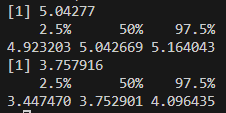
\includegraphics[width=0.7\linewidth]{img/img-2-post-summary1}
	\caption{Posterior summaries based on 10,000 iterations of Gibbs sampling (with 2,000 burn-in discarded) using a simulated dataset of size $n = 1000$ from $\mathcal{N}(5, 4)$. The posterior mean of $\mu$ is 5.04, with a 95\% credible interval of [4.92, 5.16], closely matching the true value $\mu = 5$. The posterior mean of $\sigma^2$ is 3.76, with a 95\% credible interval of [3.45, 4.10], tightly capturing the true variance $\sigma^2 = 4$.}
	\label{fig:img-2-post-summary1}
\end{figure}




\subsection{How can you use \texttt{traceplot}, the autocorrelation function and the effective sample size to determine whether the chain has converged, and whether the appropriate burn-in period has been eliminated? Use one or more of these techniques to determine whether your chain has converged and an adequate burn-in has been taken.}	

This code conducts convergence diagnostics for the output of Gibbs sampling by utilizing the \texttt{coda} package.


\begin{itemize}
	
	\item The \texttt{coda} package is loaded and the post-burn-in samples for $\mu$, $\tau$, and $\sigma^2$ are wrapped into \texttt{mcmc()} objects.
	
	\item Traceplots are generated for $\mu$ and 
	$\sigma^2$. The plots are used to visually check if mixing and convergence are occurring by observing whether a stable mean is consistently fluctuated around by the chains.
	
	\item Autocorrelation plots  are produced fofor $\mu$ and  $\sigma^2$. The Autocorrelation plots  shows how correlated samples are across lags. Rapid decay of autocorrelation indicates good mixing.
	
	\item Effective Sample Size is computed for both $\mu$ and $\sigma^2$. Effective Sample Size quantifies how many effectively independent samples are present in the chains, accounting for autocorrelation. Higher Effective Sample Size values imply better sampling efficiency and more reliable inference from the posterior distribution.
\end{itemize}

\begin{lstlisting}
	mu_chain <- mcmc(mu_post)
	tau_chain <- mcmc(tau_post)
	sigma2_chain <- mcmc(sigma2_post)
	
	#traceplota
	par(mfrow = c(2, 1))
	plot(mu_chain, main = "Traceplot of mu", col = "steelblue")
	plot(sigma2_chain, main = "Traceplot of sigma^2", col = "darkgreen")
	
	#autocorrelation plt
	par(mfrow = c(2, 1))
	autocorr.plot(mu_chain, main = "Autocorrelation Plot of mu")
	autocorr.plot(sigma2_chain, main = "Autocorrelation Plot of sigma^2")
	
	
	ess_mu <- effectiveSize(mu_chain)
	ess_sigma2 <- effectiveSize(sigma2_chain)
	
	cat("Effective Sample Size (mu):", ess_mu, "\n")
	cat("Effective Sample Size (sigma^2):", ess_sigma2, "\n")
\end{lstlisting}

\begin{figure}[H]
	\centering
	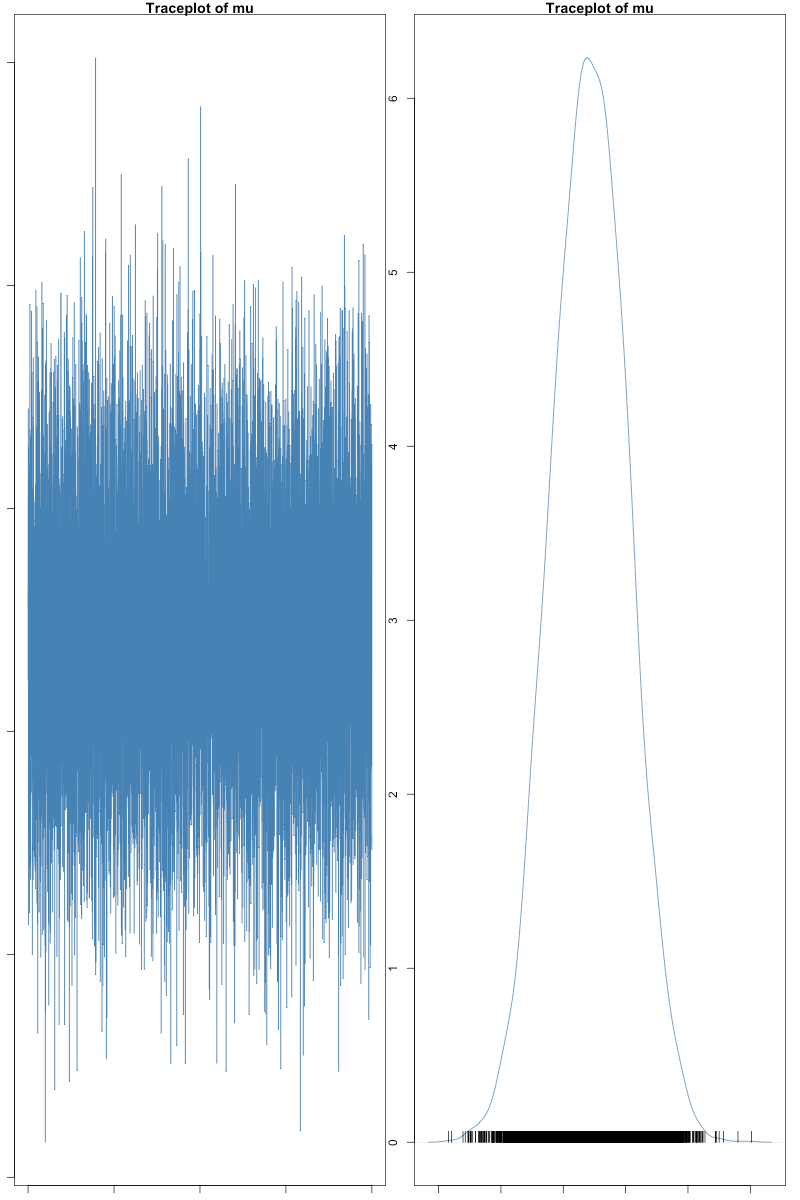
\includegraphics[width=0.7\linewidth]{img/img-traceplot-mu}
    \caption{Traceplot and posterior density plot for $\mu$. The traceplot indicates good mixing and stationarity, suggesting that the Markov chain has converged. The estimated posterior density of $\mu$,   unimodal and symmetric, with most samples concentrated around the posterior mean.}
	\label{fig:img-traceplot-mu}
\end{figure}

\begin{figure}
	\centering
	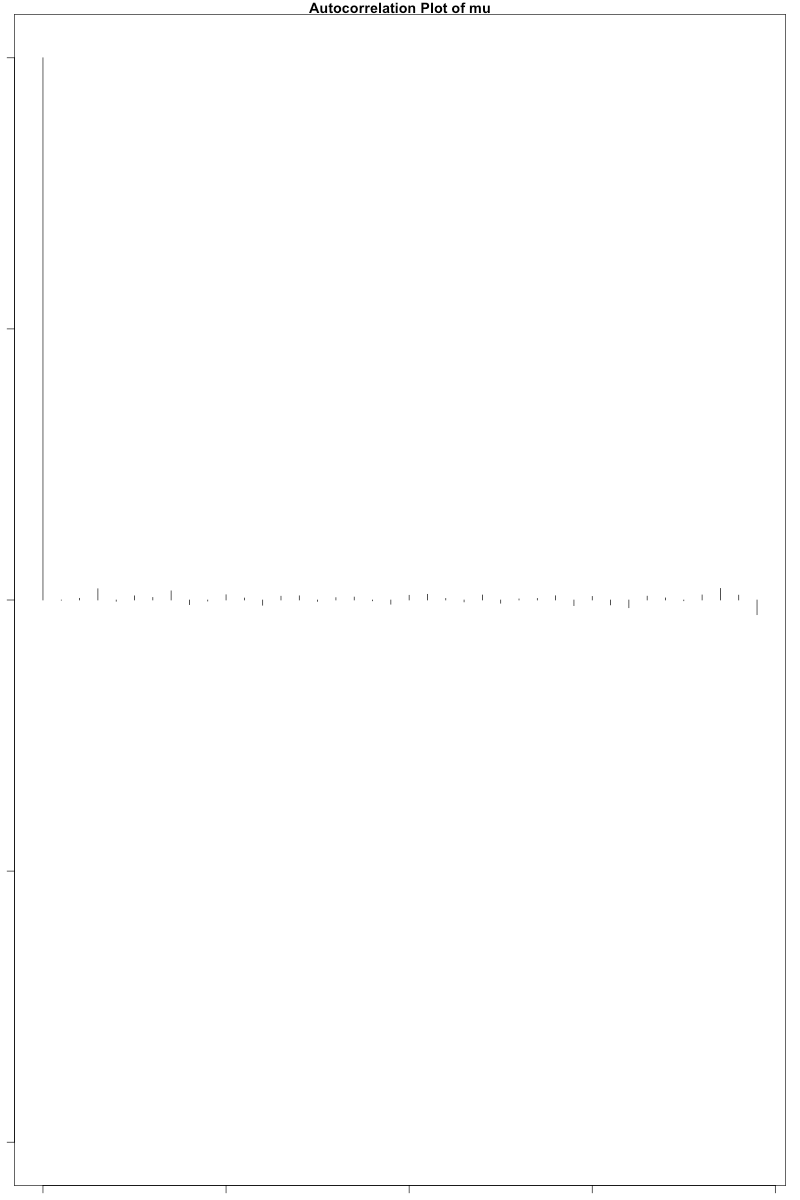
\includegraphics[width=0.7\linewidth]{img/img-autocorr-mu}
    \caption{Autocorrelation plot of the MCMC samples for $\mu$. The autocorrelation quickly drops to near zero after lag 1, indicating that the chain mixes well and successive samples are nearly independent. This suggests efficient exploration of the posterior distribution for $\mu$.}
	\label{fig:img-autocorr-mu}
\end{figure}


The trace plot of $\mu$ shows that the sampled values are well-mixed and stable. The chain quickly explores the parameter space without clear trends or drifts, which indicates it has converged well. There are no long runs of similar values, showing that the chain mixes efficiently.

The estimated distribution of $\mu$ is smooth and has a unimodal, indicating that the data is well-represented by the samples. The numerous rug ticks at the bottom of the plot show that the samples are spread evenly across the possible values.

The autocorrelation plot indicates a sharp drop after lag zero, suggesting low autocorrelation between successive samples. This is a positive sign, as it indicates that the samples in the chain are nearly independent and the Markov chain is exploring the parameter space effectively.

The reported effective sample size (ESS) for $\mu$ is 8000. Since the ESS is close to the total number of posterior draws, this confirms that the majority of samples are effectively independent. A high ESS enhances the reliability of posterior summary statistics.

The diagnostics for $\mu$ provide strong evidence of good MCMC performance. The chain has converged, exhibits efficient mixing, and has negligible autocorrelation. Therefore, the posterior estimates for $\mu$ are statistically reliable, and no further adjustments like thinning or extending the chain are necessary.


\begin{figure}[H]
	\centering
	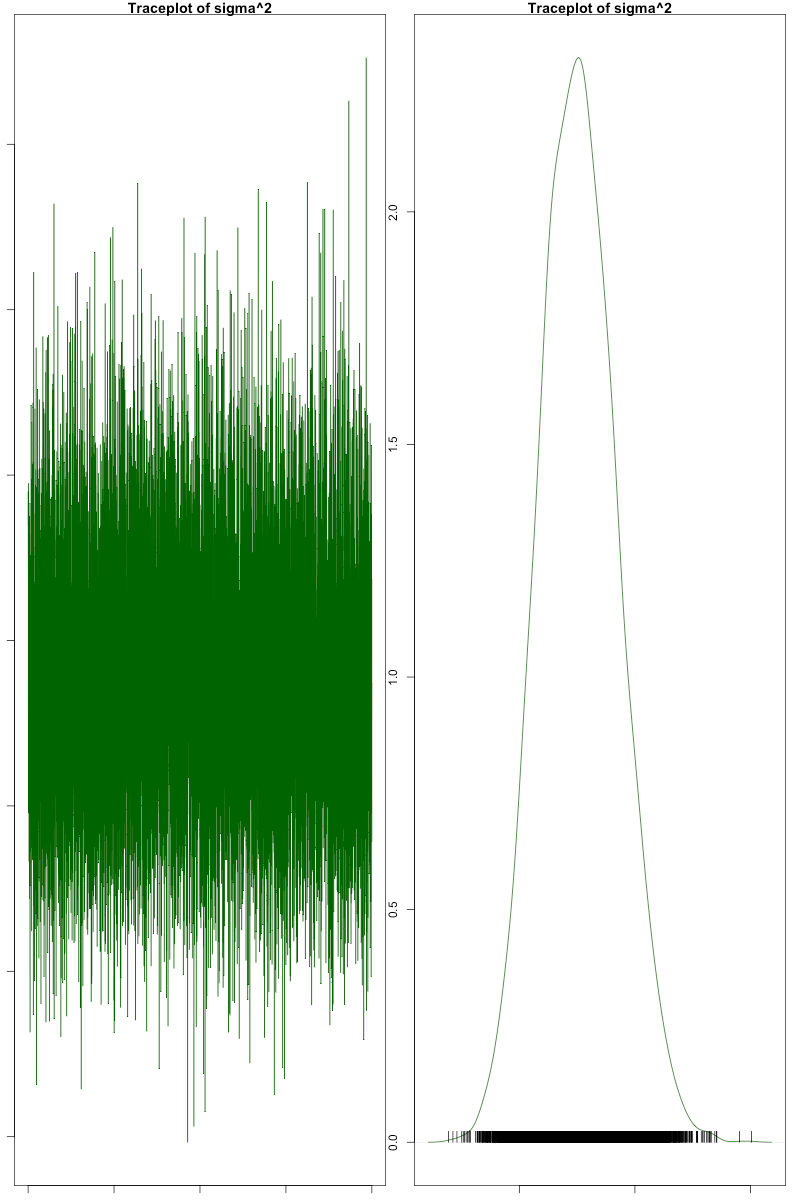
\includegraphics[width=0.7\linewidth]{img/img-traceplot-var}
    \caption{Traceplot and posterior density plot for  $\sigma^2$. The traceplot indicates good mixing and apparent stationarity of the chain, suggesting convergence to the posterior distribution. The marginal posterior density of $\sigma^2$,  is unimodal and concentrated within a narrow range, reflecting low posterior uncertainty.}
	\label{fig:img-traceplot-var}
\end{figure}



\begin{figure}[H]
	\centering
	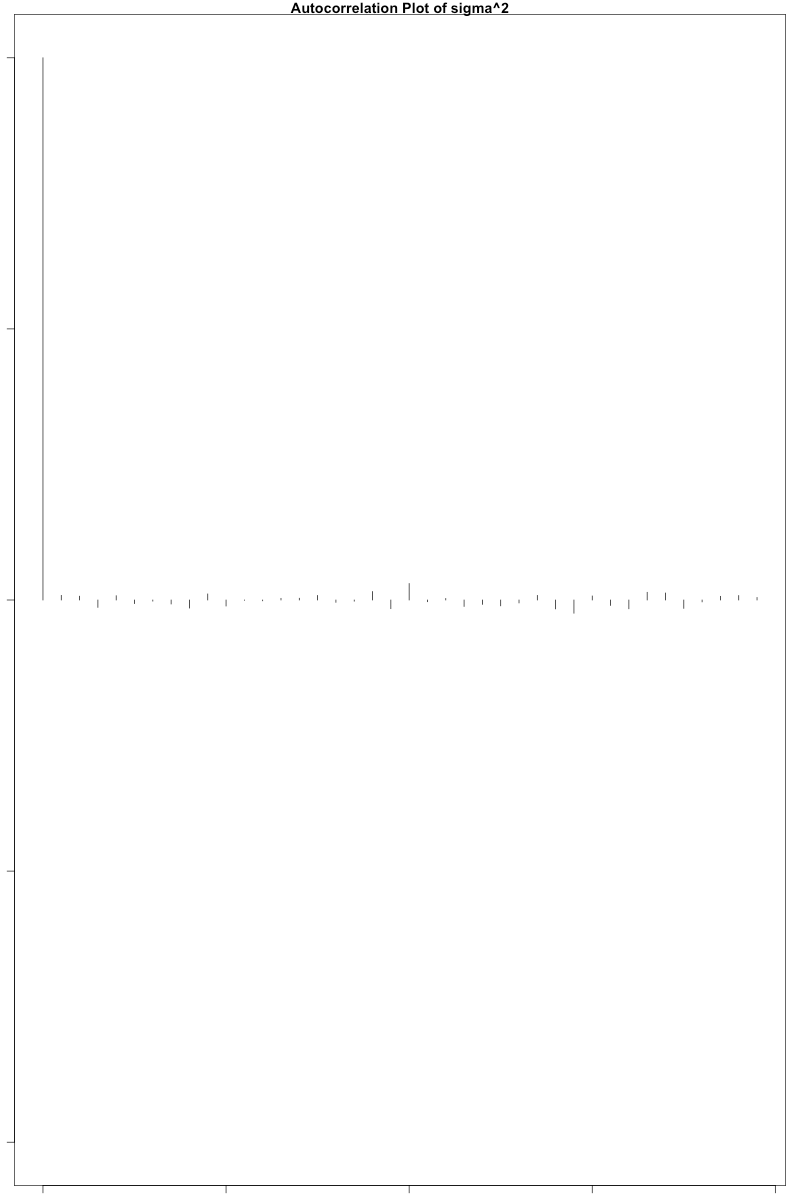
\includegraphics[width=0.7\linewidth]{img/img-autocorr-varpng}
    \caption{Autocorrelation plot of the MCMC samples for $\sigma^2$. The autocorrelation drops sharply after lag 1, indicating low serial correlation and good mixing of the Markov chain. This supports the conclusion that the posterior distribution of $\sigma^2$ has been effectively explored.}
	\label{fig:img-autocorr-varpng}
\end{figure}


\subsection{Make use of the \texttt{epdfPlot} command in the package \texttt{EnvStats} to determine the empirical pdf for $\mu$, $\tau$ and $\sigma^2$ (of course, make sure that your chain has converged and do not include the burn-in period).}


To visualise the empirical distributions of the parameters $\mu$, $\tau$, and $\sigma^2$, the \texttt{epdfPlot()} function from the \texttt{EnvStats} package in \texttt{R} was used. Posterior samples were generated using a manually implemented Gibbs sampler. The first 2000 iterations were discarded as burn-in, which allowed for the acquisition of clean posterior samples as follows:

\begin{itemize}
	\item $\mu$: directly obtained from the MCMC samples.
	\item $\tau$: sampled precision parameter.
	\item $\sigma^2$: computed as the reciprocal of $\tau$.
\end{itemize}


\begin{figure}[H]
	\centering
	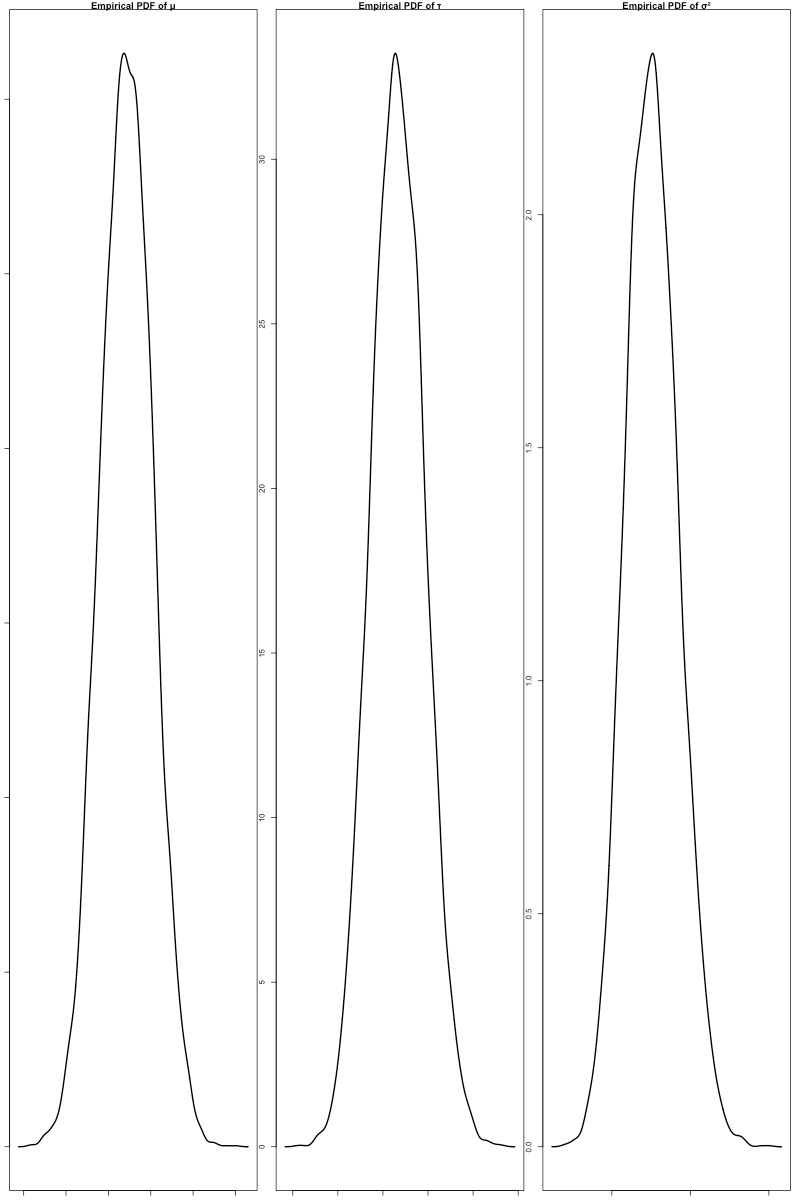
\includegraphics[width=0.7\linewidth]{img/img-endfplot}
	\caption{Empirical posterior density estimates for the parameters $\mu$, $\tau$, and $\sigma^2$, generated using the \texttt{epdfPlot()} function from the \texttt{EnvStats} package in R.}
	\label{fig:img-endfplot}
\end{figure}

The resulting empirical density plots for all three parameters were smooth, unimodal, and consistent with expectations given the large sample size and weakly informative priors. In particular:

\begin{itemize}
	\item The empirical density for $\mu$ resembles a normal distribution, reflecting low uncertainty due to the concentration of the posterior.
	\item The precision $\tau$ displayed a symmetric, bell-shaped distribution, indicating strong posterior concentration rather than prior-induced skewness.
	\item The posterior distribution of the variance $\sigma^2$ also appears symmetric, which may seem counterintuitive given that $\sigma^2$ is defined as the reciprocal of the precision parameter, $\tau$. Ordinarily, taking the inverse of a Gamma-distributed variable (such as $\tau$) results in a right-skewed Inverse-Gamma distribution for $\sigma^2$. However, in this case, the posterior distribution of $\tau$ is highly concentrated due to the large sample size ($n = 1000$), which means its variance is very small. As a result, the transformation $\sigma^2 = 1/\tau$ behaves almost linearly within the narrow range of plausible $\tau$ values. This localised linearity effectively preserves the symmetry of the distribution when mapping from $\tau$ to $\sigma^2$, resulting in a nearly symmetric posterior for $\sigma^2$ despite the nonlinear nature of the transformation.
	
\end{itemize}

These plots confirm that the MCMC simulation has effectively captured the posterior distributions of all parameters of interest.










\appendix

\section{Question 1 code} \label{appendix:a}

\begin{lstlisting}
library(rjags)
library(lattice)
library(ggplot2)
library(coda)

#load dataset
script_dir <- getwd()
concrete_cleansed_path <- file.path(
script_dir,
"project_2_code/concrete_cleansed.csv"
)
concrete_cleansed <- read.csv(concrete_cleansed_path)

jags_data <- list(
x_cement = concrete_cleansed$cement,
x_superplasticizer = concrete_cleansed$superplasticizer,
x_age = concrete_cleansed$age,
y_strength = concrete_cleansed$strength,
n = nrow(concrete_cleansed)
)

#define model
model_description <- "
model {
	for (i in 1:n) {
		y_strength[i] ~ dnorm(mu[i], tau)
		mu[i] <- beta0 +
		(beta1 * x_cement[i]) +
		(beta2 * x_superplasticizer[i]) +
		(beta3 * x_age[i])
	}
	beta0 ~ dnorm(0, 0.01)
	beta1 ~ dnorm(0, 0.01)
	beta2 ~ dnorm(0, 0.01)
	beta3 ~ dnorm(0, 0.01)
	tau ~ dgamma(0.01, 0.01)
} "

#params
n_chains <- 3
n_burnin <- 6000
n_samples <- 15000
parameters_to_monitor <- c("beta0", "beta1", "beta2", "beta3", "tau")
initial_values <- list(
list(beta0 = -10, beta1 = 0.5, beta2 = 0.1, beta3 = 0.05, tau = 0.5),
list(beta0 = 0,   beta1 = 1,   beta2 = 0.3, beta3 = 0.1,  tau = 1),
list(beta0 = 10,  beta1 = 2,   beta2 = 0.5, beta3 = 0.2,  tau = 2)
)

#create the jags model
model <- jags.model(
textConnection(model_description),
data = jags_data,
inits = initial_values,
n.chains = n_chains
)

#posterior samples from jgs model
post <- coda.samples(model = model,
variable.names = parameters_to_monitor,
n.iter = n_samples,
thin = 20)


#throw away burnin samples
post_burned <- window(post, start = n_burnin)

#posterior summary
print(summary(post_burned))

#autocorr mcmc samples
autocorr.plot(post_burned[, "beta0"])   
autocorr.plot(post_burned[, "beta1"])
autocorr.plot(post_burned[, "beta2"])
autocorr.plot(post_burned[, "beta3"])
autocorr.plot(post_burned[, "tau"])

#density plts
plot(post_burned[, "beta0"], main="beta0 -- Intercept")
plot(post_burned[, "beta1"], main="beta1 -- Cement")
plot(post_burned[, "beta2"], main="beta2 -- Superplasticizer")
plot(post_burned[, "beta3"], main="beta3 -- Age")
plot(post_burned[, "tau"], main="tau -- Precision")


print(gelman.diag(post))
gelman.plot(post_burned[, "beta0"])
gelman.plot(post_burned)



print(effectiveSize(post_burned))

#extract post samples -- generate a bunch of samples for each posterior distribution
samples_matrix <- as.matrix(post_burned)

#new values --
x_new <- c(300, 8, 28)

#compute mu for each -- scale the samples with the example values
mu_pred <- samples_matrix[, "beta0"] +
samples_matrix[, "beta1"] * x_new[1] +
samples_matrix[, "beta2"] * x_new[2] +
samples_matrix[, "beta3"] * x_new[3]

#distrib of pred mean --> distr of outcomes by adding resdl noise
tau_samples <- samples_matrix[, "tau"]
y_pred <- rnorm(length(mu_pred), mean = mu_pred, sd = 1 / sqrt(tau_samples))

print("Summary of prediction")
print(summary(y_pred))
print(quantile(y_pred, c(0.025, 0.5, 0.975)))


df <- data.frame(
predictive = y_pred,
expected = mu_pred
)


plt <- ggplot(df) +
geom_density(aes(x = predictive, color = "Predictive")) +
geom_density(aes(x = expected, color = "Expected Mean")) +
labs(title = "Posterior Predictive vs Expected Mean",
x = "Predicted Strength (MPa)",
y = "Density",
color = "Line Type") +
theme_minimal() +
scale_color_manual(values = c("Predictive" = "skyblue", "Expected Mean" = "orange")) +
scale_x_continuous(limits = c(min(df), max(df)))
print(plt)


plt <- ggplot(df, aes(x = predictive)) +
geom_density(fill = "skyblue", alpha = 0.5) +
geom_vline(aes(xintercept = mean(predictive)), color = "blue", linetype = "dashed") +
geom_vline(aes(xintercept = quantile(predictive, 0.025)), linetype = "dotted") +
geom_vline(aes(xintercept = quantile(predictive, 0.975)), linetype = "dotted") +
labs(title = "Posterior Predictive Distribution",
x = "Predicted Strength (MPa)", y = "Density") +
theme_minimal()
plot(plt)	
\end{lstlisting}


\section{Question 2 code}

\begin{lstlisting}
library(EnvStats)

## Question i

mu <- 5
sigma_2 <- 4
sigma <- sqrt(sigma_2)
n <- 1000

set.seed(1001)
x <- rnorm(n, mean = mu, sd = sigma)

# Save histogram object (does not plot automatically)
plt <- hist(x, breaks = 50, col = "skyblue", main = "Histogram of Simulated Data",
xlab = "x values", border = "white", freq = FALSE)
plot(plt)

curve(dnorm(x, mean = mu, sd = sigma), col = "blue", lwd = 2, add = TRUE)


## Question ii

m0 <- 0
v0_sq <- 1e6
a <- 0.01
b <- 0.01

## Question iii

#sampler setting
n_iter <- 10000
burn_in <- 2000

#storeage for mu and tao 
mu_samples <- numeric(n_iter)
tau_samples <- numeric(n_iter)

#init tao
tau_current <- 1 / var(x)  # start with reasonable value

x_bar <- mean(x)

for (t in 1:n_iter) {
	var_mu <- 1 / (tau_current * n + 1 / v0_sq)
	mean_mu <- var_mu * (tau_current * n * x_bar + m0 / v0_sq)
	mu_current <- rnorm(1, mean = mean_mu, sd = sqrt(var_mu))
	
	#sample tao given mu
	shape_tau <- a + n / 2
	rate_tau <- b + sum((x - mu_current)^2) / 2
	tau_current <- rgamma(1, shape = shape_tau, rate = rate_tau)
	
	#store
	mu_samples[t] <- mu_current
	tau_samples[t] <- tau_current
}

#burn-in
mu_post <- mu_samples[(burn_in + 1):n_iter]
tau_post <- tau_samples[(burn_in + 1):n_iter]
sigma2_post <- 1 / tau_post  # for inference on variance


print(mean(mu_post))
print(quantile(mu_post, c(0.025, 0.5, 0.975)))
print(mean(sigma2_post))
print(quantile(sigma2_post, c(0.025, 0.5, 0.975)))

#question iv

mu_chain <- mcmc(mu_post)
tau_chain <- mcmc(tau_post)
sigma2_chain <- mcmc(sigma2_post)

#traceplota
par(mfrow = c(2, 1))
plot(mu_chain, main = "Traceplot of mu", col = "steelblue")
plot(sigma2_chain, main = "Traceplot of sigma^2", col = "darkgreen")

#autocorrelation plt
par(mfrow = c(2, 1))
autocorr.plot(mu_chain, main = "Autocorrelation Plot of mu")
autocorr.plot(sigma2_chain, main = "Autocorrelation Plot of sigma^2")


ess_mu <- effectiveSize(mu_chain)
ess_sigma2 <- effectiveSize(sigma2_chain)

cat("Effective Sample Size (mu):", ess_mu, "\n")
cat("Effective Sample Size (sigma^2):", ess_sigma2, "\n")


# Question v

#plot the three pdfs sidebyside
par(mfrow = c(1, 3))

epdfPlot(mu_post, main = "Empirical PDF of mu")
epdfPlot(tau_post, main = "Empirical PDF of tao")
epdfPlot(sigma2_post, main = "Empirical PDF of sigma^2")

\end{lstlisting}

\end{document}
